\chapter{Interazione radiazione-materia}
	\label{chap:InterazioneRadiazioneMateria}
La quasi totalità dell'informazione di oggetti astrofisci è trasmessa tramite la radiazione elettromagnetica, usata come diagnostica della struttura fisica dell'oggetto emittente, spesso tutt'altro che banale. Un esempio è la nebulosa del granchio in figura \ref{fig:Crab}, in cui un'analisi dello spettro della parte bluastra rivela che tale radiazione sia emissione di sincrotrone, forendo utili informaizoni circa la struttura della nebulosa (campi magnetici, presenza di plasma...). La radiazione emessa dagli oggetti celesti viene di norma alterata in modo più o meno significativo nel tragitto fino a noi da materiali interposti come le polveri del \textit{mezzo interstellare} (ISM), o nebulose. A causa della dipendenza dell'assorbimento dalla lunghezza d'onda della radiazione, è possibilie caratterizzare questi materiali interposti, determinandone la composizione chimica, la densità e le dimensioni dei grani di polveri. 
Un importante fenomeno dovuto all'assorbimento consiste nell'osservazione di un gran numero di righe spettrali Lymann $\alpha$ a lunghezze d'onda maggiori di quella attesa. Ciò è dovuto agli assorbimenti della radiazione proveniente da sorgenti a grandi distanze in cui il redshift (associato all'espansione dell'universo) ha valori diversi, e quindi lo spostamento Doppler della riga Lymann $\alpha$ dipende dalla distanza a cui è avvenuto l'assorbimento. Ciò provoca una sequenza di sfasamenti Doppler della Lymann $\alpha$, nota come \textit{foresta di Lymann $\alpha$}.
\begin{figure}[b!]
\begin{center}
\includegraphics[width=0.56\textwidth]{img/crabnebula} 
\caption{Immagine della Nebulosa del Granchio.} \label{fig:Crab}
\end{center}
\end{figure}

In questo capitolo analizzeremo i principali processi di interazione radiazione-materia (tipicamente tra un fotone e un elettrone), studiando i processi di assorbimento, emissione, e scattering. Processi di assorbimento ed emissione sono processi in cui viene scambiata energia tra materia e radiazione. Tra questi ultimi si distinguono i processi \textit{free-free} (la carica è libera sia prima che dopo l'interazione con la radiazione), \textit{bound-free} (la carica si trova legata prima dell'interazione ed è libera dopo l'interazione, o viceversa), e \textit{bound-bound} (la carica è legata sia prima che dopo l'interazione con la radiazione. Ad esempio le righe spettrali sono dovute a questi processi). I processi di scattering consistono invece in una deviazione della traiettoria del fotone: tra questi si distinguono lo scattering \textit{Rayleigh}, \textit{Thomson} in cui non si ha scambio di energia tra fotone ed elettrone interagente, e scattering \textit{Compton} in cui elettrone e fotone scambiano energia durante la loro interazione. Prima di affrontare nel dettaglio questi processi, presentiamo alcuni rudimenti di elettromagnetismo per chiarire il formalismo adottato e presentare le basi della trattazione successiva. Il testo di riferimento per questo capitolo è \citep{book:Rybicki}.



\section{Radiazione}
La luce, come onda elettromagnetica, viene caratterizzata da frequenza $\nu$, frequenza angolare $\omega$, periodo $T$, lunghezza d'onda $\lambda$, numero d'onda $k$, velocità $c$. Di seguito sono riportate le principali relazioni tra queste grandezze.
\begin{align*}
\omega &= 2\pi \nu \\
T &= \inv{\nu} \\
k &= \dfrac{2\pi}{\lambda}\\
c &= \lambda\nu \approx 3\cdot 10^{10} \, \mathrm{cm}/\mathrm{s}
\end{align*}
La tabella \ref{tab:spettro} riporta la suddivisione dello spettro elettromagnetico in bande di frequenza e lunghezza d'onda, riportando inoltre i telescopi che lavorano nelle varie bande e gli oggetti tipici che emettono principalmente nella banda di interesse.
\begin{table}
\begin{center}
\begin{tabular}{ccccc}
\toprule
Banda &$\lambda$ & $\nu$ & Energia & Osservatori \\
\midrule \\[0.4ex]
Radio & $>10 \um{c}$ & $\leq 250 \uHz{M}$ &$<1\,\mu\mathrm{eV}$ & VLA, SKA \\[2pt]
Microonde & $10 \um{c} - 1 \um{m}$ & $ 250 \uHz{M} - 300 \uHz{G}$ &$1\,\mu\mathrm{eV} - 1.2 \ueV{m}$ & ALMA\\[2pt]
Infrarosso & $1 \um{m} - 700 \um{n}$ & $ 300 \uHz{G} - 428 \uHz{T}$ &$ 1.2 \ueV{m} - 1.8 \ueV{}$ & Spitzer, Hershel\\[2pt]
Visibile & $700 \um{n} - 400 \um{n}$ & $ 428 \uHz{T} - 749 \uHz{T}$ &$1.8 \ueV{} - 3.1 \ueV{}$ & Hubble, VLT\\[2pt]
Ultravioletto & $400 \um{n} - 10 \um{n}$ & $ 749 \uHz{T} - 30 \uHz{P}$ &$3.1 \ueV{} - 124 \ueV{}$ & Hubble\\[2pt]
X& $10 \um{n} - 1 \um{p}$ & $ 30 \uHz{P} - 300 \uHz{E}$ &$124 \ueV{} - 1.24 \ueV{M}$ & Swift, Chandra, ATHENA\\[2pt]
Gamma& $< 1 \um{p}$ & $ > 300 \uHz{E}$ &$>1.24 \ueV{M}$ & IACT\\[2pt]
\bottomrule
\end{tabular} 
\end{center}
\caption{La tabella riporta la principale suddivisione dello spettro elettromagnetico, indicando le energie associate e i più importanti strumenti che operano in tali bande.} \label{tab:spettro}
\end{table}



\subsection{Equazioni di Maxwell}\label{sec:EqMaxwell}
In questo corso adotteremo il sistema $cgs$: le equazioni di Maxwell in questo sistema sono
\begin{EQ}
\begin{equation}
\begin{cases}
\Div{D} = 4\pi\rho \\
\Div{B} = 0 \\
\Rot{E} = -\inv{c}\derP{\V{B}}{t} \\[10pt]
\Rot{H} = \inv{c}\derP{\V{D}}{t} + \dfrac{4\pi}{c} \V{J}
\end{cases} \label{eq:Maxwell1}
\end{equation}
\end{EQ}
dove $\V{D}$ è il campo di induzione elettrica, $\rho$ è la densità di carica elettrica, $\V{B}$ è il campo di induzione magnetica, $\V{E}$ è il campo elettrico mentre $\V{H}$ è il campo magnetico. Le relazioni tra i campi di induzione e i campi sono
\begin{equation}
\begin{cases}
\V{D}= \varepsilon \V{E} \\
\V{B}=\mu \V{H}
\end{cases}
\end{equation}
dove $\varepsilon$ è la costante dielettrica, mentre $\mu$ è la permeabilità magnetica. Nel sistema cgs sono costanti adimensionali che valgono $1$ nel vuoto. Notiamo inoltre che in questo sistema campo elettrico e magnetico hanno le stesse dimensioni. In questo caso le equazioni si riducono a
\begin{EQ}
\begin{equation}
\begin{cases}
\Div{E} = 0 \\
\Div{B} = 0 \\
\Rot{E} = -\inv{c}\derP{\V{B}}{t} \\[10pt]
\Rot{B} = \inv{c}\derP{\V{E}}{t} 
\end{cases} \label{eq:Maxwell2}
\end{equation}
\end{EQ}
 Combinando le equazioni di Maxwell si ottiene l'equazione di continuità della carica elettrica
\begin{EQ}
\begin{equation}
\derP{\rho}{t} + \Div{J} =0
\end{equation}
\end{EQ}
Concettualmente si può dire che le equazioni di Maxwell mostrano come le cariche generano i campi; il modo in cui i campi agiscono su una carica è invece espresso dalla forza di Lorentz
\begin{EQ}
\begin{equation}
\V{F} = q\left(\V{E} + \dfrac{\V{v}}{c}\times\V{B}\right) \label{eq:Lorentz}
\end{equation}
\end{EQ}
dove $q$ indica la carica singola.
Possiamo esprimere la forza di Lorentz per unità di volume
\begin{equation}
\V{f} = \rho\V{E} + \dfrac{\V{J}}{c}\times\V{B}
\end{equation}
Possiamo ora calcolare la potenza erogata dal campo elettromagnetico per accelerare una carica $q$. 
\begin{equation}
\der{W}{t} = \scal{f}{v} =\footnote{Questo mostra che il lavoro è fatto dal solo campo elettrico, non da quello magnetico.} \rho \scal{v}{E} = \scal{J}{E} =\footnote{In questo passaggio sostituiamo la quarta equazione di Maxwell.} \dfrac{c}{4\pi}(\Rot{H})\cdot\V{E} - \inv{4\pi}\derP{\V{D}}{t}\cdot\V{E} 
\end{equation}
Sfruttando la proprietà $\Div{}(\vett{A}{C}) = \scal{C}{}(\Rot{A})-\scal{A}{}(\Rot{C})$ otteniamo
\begin{equation}
\der{W}{t} = \dfrac{c}{4\pi}\Div{}(\vett{H}{E}) + \dfrac{c}{4\pi} \scal{H}{}(\Rot{E}) -\inv{4\pi} \derP{\V{D}}{t}\scal{}{E} = \dfrac{c}{4\pi}\Div{}(\vett{H}{E}) - \inv{8\pi} \derP{}{t}(\scal{B}{H}+\scal{D}{E})
\end{equation}
dove nell'ultimo passaggio abbiamo utlizato la terza equazione di Maxwell e raccolto i termini con derivata temporale. A questo punto definendo 
\begin{EQ}
\begin{align}
&\V{S} \equiv \dfrac{c}{4\pi} \vett{E}{H}
&U \equiv \inv{8\pi}(\scal{E}{D} + \scal{B}{H})
\end{align}
\end{EQ}
otteniamo un importante risultato dell'elettromagnetismo
\begin{EQ}
\begin{equation}
\derP{\V{U}}{t}+\Div{S} = - \der{W}{t}
\end{equation}
\end{EQ}
Questa equazione è l'equazione di continuità della grandezza $U$, ovvero la densità di energia del campo elettromagnetico. Il flusso di questa quantità e il \textit{vettore di Poynting} $\V{S}$. Vediamo che nell'accelerare una carica, il campo elettromagnetico perde energia.

Un altro importante risultato dell'elettromagnetismo è ottenibile combinando le equazioni \ref{eq:Maxwell2}, sfruttando le identità degli operatori vettoriali:
\begin{equation}
\Rot{}(\Rot{E})=\Grad(\Div{E}) - \Grad^2\V{E} = -\inv{c}\derP{}{t}(\Rot{B}) = -\inv{c^2}\derPn{\V{E}}{t}{2}
\end{equation}
Procedendo analogamente per $\V{B}$ otteniamo le equazioni delle onde per il campo elettrico e magnetico
\begin{EQ}
\begin{align}
&\Grad^2 \V{E} -\inv{c^2}\derPn{\V{E}}{t}{2} = 0
&\Grad^2 \V{B} -\inv{c^2}\derPn{\V{B}}{t}{2} = 0
\end{align}
\end{EQ}
le cui soluzioni sono onde piane del tipo
\begin{EQ}
\begin{align}
&\V{E}=\V{E}_0 e^{i(\scal{k}{r}-\omega t)}
&\V{B}=\V{B}_0 e^{i(\scal{k}{r}-\omega t)}
\end{align}
\end{EQ}
Questo risultato mostra che nel vuoto le variazioni del campo elettrico e magnetico si autosostengono, propagando come onde dette onde elettromagnetiche. Sostituendo le onde piane nelle prime due equazioni di Maxwell si trova che $\scal{k}{E}_0=0$ e $\scal{k}{B}_0=0$ cioè che le onde elettromagnetiche sono trasversali alla direzione di propagazione. Infine sostituendo le onde piane nelle ultime due equazioni si trova 
\begin{align}
&\vett{k}{E}_0 = \dfrac{\omega}{c} \V{B}_0
&\vett{k}{B}_0 = \dfrac{\omega}{c} \V{E}_0
\end{align}
che implica che il campo elettrico e il campo magnetico dell'onda sono ortogonali tra loro; inoltre dalle due relazioni precedenti si ottiene la relazione di dispersione delle onde elettromagnetiche, $\omega^2=k^2c^2$, da cui risulta che nel vuoto i moduli del campo elettrico e magnetico sono uguali, ovvero $\V{E}_0=\V{B}_0$. Da ciò segue anche che 
\begin{EQ}
\begin{align}
&U\inv{4\pi}E_0^2 = \inv{4\pi}B_0^2
&\V{S} = \dfrac{c}{4\pi} E_0^2 \vers{k} = Uc\vers{k}
\end{align}
\end{EQ}
L'ultima uguaglianza mostra che il flusso del campo elettromagnetico (il vettore di Poynting) è dato dalla densità di energia per la velocità della luce (velocità di propagazione dell'onda) nella direzione di propagazione $\vers{k}$.

Se la variazione di direzione di $\zeta$ (vettore funzione d'onda) nel piano ortogonale alla propagazione in funzione della coordinata spaziale di propagazione e del tempo può essere espressa da una legge (funzione), si dice che l'onda è polarizzata. 
In generale un'onda elettromagnetica è data dalla sovrapposizione di più onde, non necessariamente in fase tra loro
\begin{equation}
\V{E}=\V{E}_1 e^{i\omega t} + \V{E}_2 e^{i\omega t} e^{i\phi}
\end{equation}
dove i campi $\V{E}_1$ e $\V{E}_2$ contengono l'ampiezza e il termine di propagazione spaziale. Se $\V{E}_1=\V{E}_2$ e $\phi=0$ l'onda è polarizzata linearmente, ovvero i campi oscillano su una linea appartenente al piano ortogonale alla direzione di propagazione. Se $\V{E}_1=\V{E}_2$ e $\phi = \pm \pi/2$ la polarizzazione è circolare: se $\phi=+\pi/2$ si ha polarizzazione sinistra (il vettore ruota in senso antiorario), se $\phi=-\pi/2$ si ha polarizzazione destra (il vettore ruota in senso orario). Infine se $\V{E}_1\neq\V{E}_2$ ma $\phi = \pm \pi/2$ l'onda ha polarizzazione ellittica. 
Il caso ancora più generico è quello in cui il campo è dato dalla sovrapposizione di più onde a frequenze $\omega$ differenti.

\subsection{Spettro}
Con \textit{spettro di una radiazione} si indica l'insieme delle frequenze di cui è composta la radiazione elettromagnetica osservata.
Lo spettro della radiazione dipende dalla variazione temporale del campo elettrico (ignoriamo per semplicità il campo magnetico poichè le sue variazioni dipendono da quelle del campo elettrico). Una conseguenza di ciò è che non è possibiile dare un significato preciso allo spettro di una radiazione in un dato istante di tempo sapendo solo il campo elettrico in un punto. Occorre invece parlare di spettro di un treno d'onda o di radiazione in un punto in un lungo intervallo di tempo $\Delta t$. Se si dispone di un tempo di osservazione del campo della radiazione $\Delta t$, è possibile definire lo spettro con una risoluzione di frequenza $\Delta \omega$, con $\Delta \omega \, \Delta t >1$. Questa relazione di indeterminazione non è necessariamente quantistica, ma è comunque una proprietà alla base di ogni teoria ondulatoria della luce. Questa relazione implica che quanto più grande è il tempo di osservazione della radiazione, tanto più sarà dettagliata la nostra conoscenza dello spettro, ovvero della frequenza $\Delta\omega$.


%Assumioamo per semplicità matematica, che la radiazione sia nella forma di un impulso finito (in pratica richiediamo che il campo elettrico $\V{E}(t)$ si annulli rapidamente per $t\longrightarrow\pm\infty$). Inoltre 

Prima di discutere lo spettro della radiazione, ricordiamo che data una funzione del tempo $a(t)$, è possibile esprimerla in termini della trasformata di Fourier $\tilde{a}(\omega)$
\begin{EQ}
\begin{align}
&a(t) = \int_{-\infty}^{+\infty}\tilde{a}(\omega)\,e^{-i\omega t} \dd\omega
&\tilde{a}(\omega) = \inv{2\pi}\int_{-\infty}^{+\infty}a(t)\,e^{i\omega t} \dd t
\end{align}
\end{EQ}
Ricordiamo il teorema di Parseval
\begin{EQ}
\begin{equation}
\int_{-\infty}^{+\infty} a^2(t) \dd t = 2 \pi \int_{-\infty}^{+\infty} |\tilde{a}(\omega)|^2 \dd \omega
\end{equation}
\end{EQ}
Inoltre un'utile proprietà è che se $a(t)$ è reale, allora si ha
\begin{align}
\tilde{a}(-\omega) &= \inv{2\pi} \int_{-\infty}^{+\infty} a(t)\, e^{-i\omega t} \dd t = \\
&=\inv{2\pi} \int_{-\infty}^{+\infty} a^*(t)\, e^{-i\omega t} \dd t = \\
&= \tilde{a}^{*}(\omega) \label{eq:Spettro1}
\end{align}
dove $*$ indica il complesso coniugato. 

La trasformata di Fourier del campo elettrico $\hat{\V{E}}(\omega)$ contiene tutte le informazioni sulla dipendenza dalla frequenza del campo elettrico $\V{E}(t)$; infatti non è altro che il campo elettrico nel dominio delle frequenze. Per ottenere la dipendenza dalla frequenza dell'energia della radiazione, possiamo scrivere il flusso della radiazione (cioè l'energia che transita attraverso la superficie unitaria nell'unità di tempo) tramite il vettore di Poynting
\begin{equation}
\dfrac{\dd W}{\dd t \, \dd A} =  |\V{S}| = \dfrac{c}{4 \pi} |\V{E}(t)|^2
\end{equation}
A questo punto integriamo su tutti i tempi, e sfruttando il teorema di Parseval e la proprietà \ref{eq:Spettro1}, otteniamo
\begin{equation}
\der{W}{A} = \dfrac{c}{4\pi} \int_{-\infty}^{+\infty} |\V{E}(t)|^2 \dd t = \dfrac{c}{2} \int_{-\infty}^{+\infty} |\hat{\V{E}}(\omega)|^2 \dd \omega = c \int_{0}^{+\infty} |\hat{\V{E}}(\omega)|^2 \dd \omega
\end{equation}
Possiamo così identificare l'energia per unità di area e di frequenza con
\begin{EQ}
\begin{equation}
\dfrac{\dd W}{\dd A \, \dd \omega} = c |\hat{\V{E}}(\omega)|^2
\end{equation}
\end{EQ}
Sottolineaiamo il fatto che questa è l'energia totale per unità di area e di frequenza di un intero impulso; non abbiamo scritto "per unità di tempo". Infatti per scrivere sia $\dd t$ che $\dd\omega$ violeremmo il principio di indeterminazione tra $\omega$ e $t$. Tuttavia se l'impulso si ripete con un periodo $T$, allora è possibile scrivere formalmente 
\begin{equation}
\dfrac{\dd W}{\dd A \, \dd \omega \, \dd t} \equiv \inv{T} \dfrac{\dd W}{\dd A \, \dd \omega} = \dfrac{c}{T} |\V{E}(\omega)|^2
\end{equation}
Questa formula può essere usata per definire lo spettro di una porzione di lunghezza $T$ di un segnale molto più lungo. Se un segnale ha più o meno le stesse proprietà lungo tutta la sua durata (cioè è stazonario), allora ci aspettiamo che il risultato sia indipendente da $T$ per grandi $T$, e possiamo scrivere
\begin{equation}
\dfrac{\dd W}{\dd A \, \dd \omega \, \dd t}  = c \lim_{T\to\infty} \inv{T} |\hat{\V{E}}_T(\omega)|^2
\end{equation}
dove la scrittura $\hat{\V{E}}_T(\omega)$ serve a enfatizzare il fatto che è la trasformata di Fourier di una porzione di lunghezza $T$ della funzione $\V{E}$. In questo modo possiamo generalizzare la discussione fino ad includere onde infinitamente lunghe (come onde sinusoidali) usando formule basate su quelle ottenute per un impulso finito. Se le proprietà di $\V{E}(t)$ variano nel tempo, ci sia aspetta che lo spettro determinato dall'analisi di una porzione di lunghezza $T$ dipenda solo dalla porzione analizzata. In questo caso il concetto di spettro locale avrà senso se la variazione del campo $\V{E}(t)$ avviene su una scala temporale abbastanza lunga da poter definire un intervallo $T$ in cui si può ottenere una risoluzione di frequenza $\Delta \omega$ tale che $\Delta\omega \sim 1/T$. Se questa condizione non è soddisfatta la definizione di uno spettro locale non è utile, e occorre considerare lo spettro di tutto l'impulso come entità di base. Consideriamo ora alcuni impulsi tipici e i loro spettri corrispondenti (figura \ref{fig:Impulso1}, \ref{fig:Impulso2}, \ref{fig:Impulso3}). Studi come questo permettono di ottenere informazioni sulle relazioni utili nella stima degli spettri di un particolare processo. Notiamo che l'estensione dell'impulso $T$ determina la larghezza della più fine struttura risolvibile nello spettro: più grande è $T$, più stretto è il picco nel dominio delle frequenze. Inoltre notiamo che una dipendenza sinusoidale dal tempo causa un picco nel dominio delle frequenze centrato in $\omega_0$. Per $T\to\infty$ (dove, ricordiamo, $T$ è il tempo di osservazione dell'impulso, non il periodo della sinusoide) lo spettro tende ad una delta di Dirac centrata in $\omega_0$.
\begin{figure}
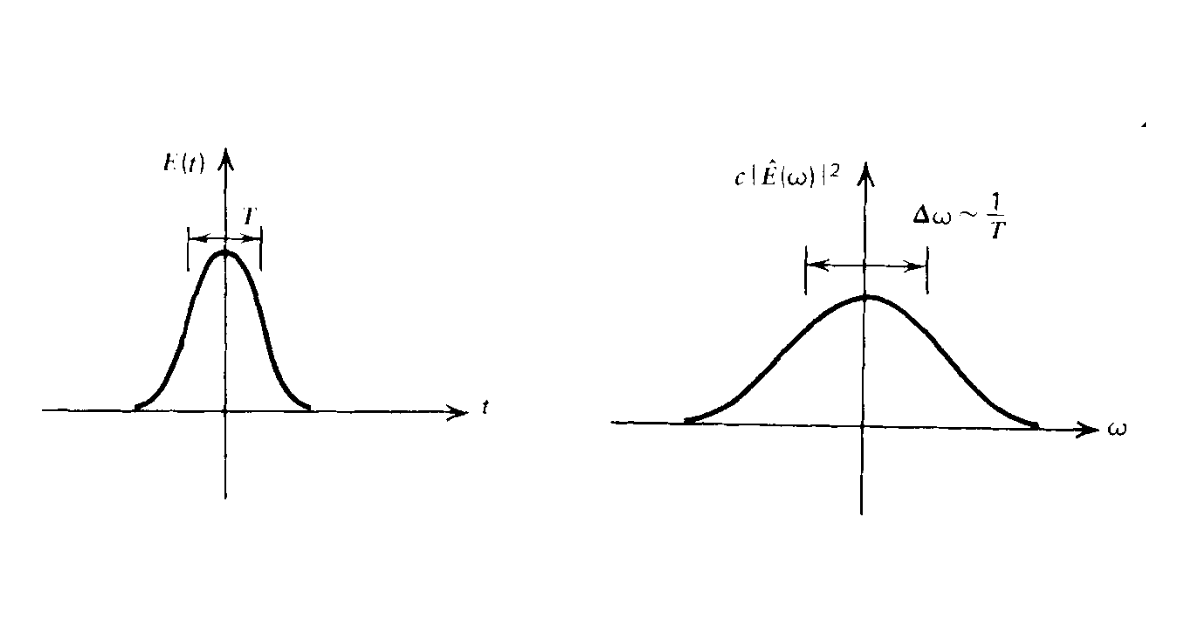
\includegraphics[width=\textwidth]{img/Impulso1}
\caption{Impulso gaussiano di larghezza $T$.}\label{fig:Impulso1}
\end{figure}
\begin{figure}
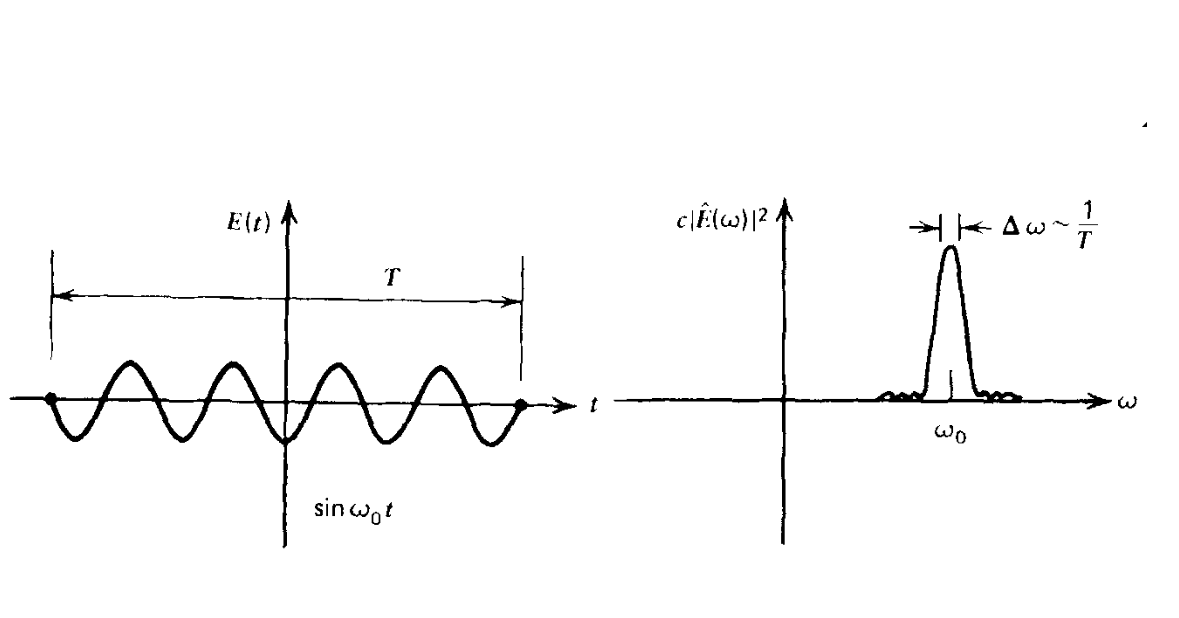
\includegraphics[width=\textwidth]{img/Impulso2}
\caption{Impulso sinusoidale $\sin \omega_0 t$.}\label{fig:Impulso2}
\end{figure}
\begin{figure}
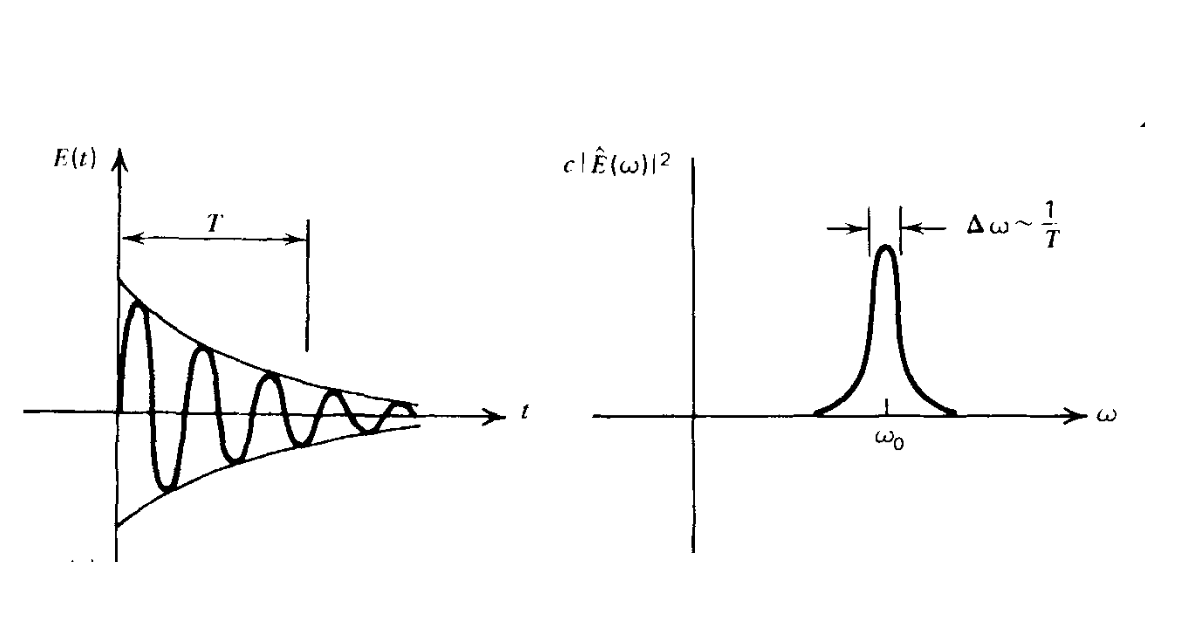
\includegraphics[width=\textwidth]{img/Impulso3}
\caption{Impulso sinusoidale con smorzamento $\exp{-t/T}$.}\label{fig:Impulso3}
\end{figure}

\section{Radiazione da carica accelerata}
La derivazione canonica delle equazioni che descrivono la radiazione generata da una carica accelerata parte dalle equazioni di Maxwell e richiede di scrivere i potenziali ritardati del campo elettrico e magnetico, in un punto distante $\V{r}$ dalla carica. È tuttavia più istruttivo seguire l'approccio di Thomson \citep{book:Longair}, che mostra più chiaramente l'origine fisica della radiazione di una carica accelerata.

Consideriamo una carica $q$ stazionaria nell'origine $O$ di un sistema di riferimento inerziale $S$ al tempo $t=0$. Supponiamo che la carica subisca una piccola accelerazione alla velocità $\Delta v$ in un breve intervallo di tempo $\Delta t$. Thomson visualizzò il campo risultante in termini delle linee di campo, come mostrato in figura \ref{fig:Radiazione1}.
\begin{figure}
\begin{center}
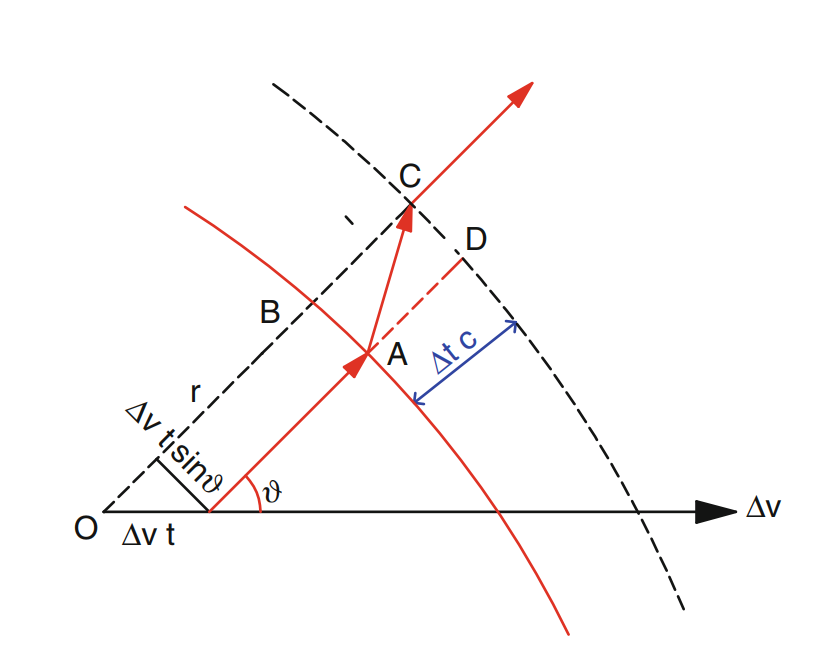
\includegraphics[width=0.8\textwidth]{img/CaricaAccelerata}
\caption{Schema delle linee di campo associate ad una carica accelerata. La figura è discussa nel testo.} \label{fig:Radiazione1}
\end{center}
\end{figure}
Dopo un tempo $t$ possiamo distinguere tra la configurazioni dentro e fuori la sfera di raggio $r=ct$ centrata in $O$ poichè le perturbazioni del campo elettromagnetico propagano a velocità $c$ nel vuoto. Fuori dalla sfera, l'informazione dello spostamento della carica da $O$ non è ancora pervenuta, poichè appunto tale informazione viaggia alla velocità della luce. Tra queste due regioni abbiamo un sottile guscio di spessore $c\Delta t$ in cui si devono congiungere le corrispondenti linee di campo. Geometricamente è chiaro che ci deve essere una componente del campo elettrico in direzione tangenziale, ovvero in direzione $\hat{\V{\theta}}$. L'impulso del campo elettromagnetico è propagato dalla carica a velocità $c$, e corrisponde alla perdita di energia impiegata per accelerare la carica. 
Studiamo ora questo impulso del campo elettrico che sta propagando nello spazio. Assumiamo anzitutto che l'incremento di velocità $\Delta v$ subito dalla carica sia molto piccolo, ($\Delta v \ll c$, ovvero regime non relativistico), potendo così assumere che le linee di campo sono radiali nel sistema $S$ non solo a $t=0$ ma anche al tempo $t$. Consideriamo la linea di campo ad un angolo $\theta$; congiungiamo le linee di campo attraverso il guscio di spessore $c\Delta t$. Dalla geometria del sistema risulta che 
\begin{equation}
\dfrac{{E}_\theta}{{E}_r} = \dfrac{\Delta v \, t \sin \theta}{\Delta t \,c} = \dfrac{a\,r}{c^2} \sin\theta
\end{equation}
dove $a$ è il modulo dell'accelerazione subita dalla carica. Essendo poi noto il campo radiale $\V{E}_r = q/r^2 \,\V{r}$, otteniamo il \textit{campo di radiazione}
\begin{EQ}
\begin{equation}
E_\theta = \dfrac{q \,a}{rc^2} sin\theta
\end{equation}
\end{EQ}
Notiamo che la componente radiale del campo decresce come $r^{-2}$, in accordo con la legge di Coulomb, mentre la componente tangenziale decresce solo come $r^{-1}$; ciò è in accordo col fatto che l'intensità di un'onda (ovvero il suo vettore di Poynting) è proporzionale a $E^2$ e che l'intensità di un'onda sferica decresce come $r^{-2}$. Notiamo infine che il modulo del campo di radiazione è direttamente proporzionale all'acelerazione della carica, e dipende dall'angolo considerato (si ha un minimo nella direzione dell'accelerazione e un massimo nella direzione ortogonale all'accelerazione).
Consideriamo ora $\vers{n}$ direzione di propagazione, e indichiamo con il pedice rad i campi di radiazione: geometricamente si ha
\begin{align}
&\V{E}_\mathrm{rad} = \dfrac{q}{rc^2} \vers{n}\times(\vett{\hat{n}}{a})
&\V{B}_\mathrm{rad} = \vers{n}\times \V{E}_\mathrm{rad} = - \dfrac{(\vett{\hat{n}}{a})q}{rc^2}
\end{align}
In generale il campo radiativo al tempo $t$ è funzione dell'accelerazione calcolata al tempo $(t-r/c)$ poichè l'informazione contenuta nel guscio sferico propaga a velocità $c$. Possiamo ora calcolare il vettore di Poynting, ottenendo la \textit{formula di Larmor} per unità di superficie
\begin{EQ}
\begin{equation}
\dfrac{\dd W}{\dd t \, \dd A} = |\V{S}| = \dfrac{c}{4\pi} E_\mathrm{rad}^2 = \dfrac{q^2 |\vett{\hat{n}}{a}|^2}{4\pi c^3 r^2} = \dfrac{q^2 a^2 \sin^2 \theta}{4\pi c^3 r^2} \label{eq:Larmor1}
\end{equation}
\end{EQ}
Riascivendo l'equazione in termini di angolo solido\footnote{La definizione di angolo solido è $\dd \Omega = \dfrac{\dd A}{r^2}$} otteniamo la \textit{formula di Larmor}
\begin{EQ}
\begin{equation}
\dfrac{\dd W}{\dd t \, \dd \Omega} = r^2|\V{S}| =\dfrac{q^2 |\vett{\hat{n}}{a}|^2}{4\pi c^3} = \dfrac{q^2 a^2 \sin^2 \theta}{4\pi c^3} \label{eq:Larmor2}
\end{equation}
\end{EQ}
Un'altra forma della formula di Larmor è quella ottenuta integrando su tutti gli angoli solidi. Il risultato fornisce la potenza totale emessa
\begin{EQ}
\begin{equation}
\der{W}{t} = \dfrac{2}{3} \dfrac{q^2 a^2}{c^3} \label{eq:Larmor3}
\end{equation}
\end{EQ}
La formula di Larmor, sia in forma differenziale che integrale, mostra che la potenza emessa è porporzionale al quadrato della carica e dell'accelerazione. Inoltre essa ha l'andamento tipico del dipolo ovvero la proporzionalità a $\sin^2 \theta$; non si ha emissione di radiazione lungo la direzione dell'accelerazione, e il massimo dell'emissione è in direzione perpendicolare all'accelerazione. 

Quando abbiamo a che fare con $N$ particelle in diverse posizioni $\V{r}_i$, velocità $\V{v}_i$ e carica $q_i$, possiamo calcolare il campo a grandi distanze semplicemente sovrapponendo tra loro i singoli $\V{E}_\mathrm{rad}$ associati a ciascuna particella. Tuttavia si ha una complicazione dovuta al fatto che la formula di Larmor ottenuta si riferisce a condizioni a tempi ritardati, e ciascuna particella ha tempi ritardati diversi. Un altro modo di vedere questa complicazione è che nel sovrapporre i campi di radiazione delle singole particelle dobbiamo tener conto delle differenze di fase dei diversi campi introdotte dai ritardi (causati dal fatto che le particelle occupano posizioni diverse). Questa complicazione può però essere eliminata soto opportune ipotesi. Supponiamo che il sistema abbia dimensione tipica $L$, e che la scala temporale su cui avviene l'accelerazione delle cariche sia $\tau$. Se $\tau\gg L/c$, ovvero se il tempo scala è molto più grande del tempo che la luce impiega a coprire la distanza tipica del sistema di cariche, allora le differenze tra i tempi di ritardo della sorgente sono trascurabili. Possiamo anche caratterizzare il tempo $\tau$ come la scala temporale oltre la quale si hanno cambiamenti significativi nel campo radiativo, scala temporale che determina la tipica frequenza della radiazione emessa. Chiamando $\nu$ tale frequenza si ha che $\nu = \tau^{-1}$. L'approssimazione $\tau\gg L/c$ può quindi essere riscritta come $\lambda\gg L$ con $\lambda$ lunghezza d'onda della radiazione. Pertanto se il sistema è piccolo in confronto alla l'unghezza d'onda della radiazione emessa, è possibile ignorare le differenze i ritardi temporali e quindi le differenze di fase tra i campi di radiazione dovuti alle singole cariche e calcolare il campo di radiazione totale come
\begin{equation}
\V{E}_\mathrm{rad} = \sum_{i=1}^N \dfrac{\vers{n}\times(\vett{\hat{n}}{\ddot{d}_i})}{r_i\, c^2}
\end{equation}
dove $\ddot{d}$ è la derivata temporale seconda del momento di dipolo elettrico della associato alla carica i-esima. Se siamo in \textit{approssimazione di dipolo}, ovvero se valgono le condizioni $\tau\gg L/c$ e $R\gg L$, con $R$ distanza dall'oggetto emittente si ha 
\begin{EQ}
\begin{equation}
\V{E}_\mathrm{rad} = \dfrac{\vers{n}\times(\vett{\hat{n}}{\ddot{D}})}{R\, c^2}
\end{equation}
\end{EQ}
avendo definito
\begin{equation}
\V{D}= \sum_{i=1}^N d_i
\end{equation}
Infine si può dimostrare (vedi \cite{book:Rybicki}) che l'energia emessa per unità di frequenza è 
\begin{EQ}
\begin{equation}
\der{W}{\omega} = \dfrac{8\pi}{3} \dfrac{\omega^4}{c^3} |\tilde{D}(\omega)|^2 \label{eq:Larmor4}
\end{equation}
\end{EQ}
dove $\tilde{D}(\omega)$ indica la trasformata di Fourier del momento di dipolo totale.

\subsection{Radizione di ciclotrone}\label{subsec:Ciclotrone}
Il ciclotrone è il caso relativistico del sincrotrone, trattato nella sezione \ref{subsec:Sincrotrone}, e consiste in una carica (tipicamente un elettrone, motivo per cui interscambieremo il termine carica con elettrone) in moto in un campo magnetico costante $\V{B}$. La carica $q$ di massa $m$ subisce un'accelerazione dovuta alla forza di Lorentz \ref{eq:Lorentz}. Per semplicità supponiamo che la carica si muova in un piano ortogonale al campo magnetico, orientato lungo $\vers{z}$. Otteniamo il sistema
\begin{align}
&\begin{cases}
m\,a_x &=  \dfrac{q \, B\, v_y}{c} \\[10pt]
m\,a_y &=  \dfrac{q \, B\, v_x}{c}
\end{cases}
&\Longrightarrow \,\,\,\,\,\,\,\,\,\,\,\,\,\,\,\,\,\,\,\,\,\,\,\,\,\,
&\begin{cases}
\ddot{v}_x &= -\left(\dfrac{q\, B\,}{m\, c}\right)^2 v_x \\[10pt]
\ddot{v}_y &= -\left(\dfrac{q\, B\,}{m\, c}\right)^2 v_y
\end{cases}
\end{align}
e si definisce la frequenza di ciclotrone come 
\begin{EQ}
\begin{equation}
\omega_\mathrm{c} = \dfrac{q\, B\,}{m\, c}
\end{equation}
\end{EQ}
Possiamo calcolare la potenza emessa sfruttando la formula di Larmor \ref{eq:Larmor3} (ponendo $a= \omega_\mathrm{c} v$) e definendo $\beta \equiv v/c $ otteniamo
\begin{equation}
\der{W}{t} = \dfrac{2}{3} r_0^2 \, c\,\beta^2\, B^2
\end{equation}
avendo definito 
\begin{equation}
r_0 \equiv \dfrac{q^2}{m c^2}
\end{equation}
raggio classico dell'elettrone, ovvero la distanza a cui il potenziale elettrostatico è uguale all'energia a riposo dell'elettrone. Se definiamo la densità di energia del campo magnetico $U_B$
\begin{equation}
U_B \equiv \dfrac{B^2}{8\pi}
\end{equation}
e la \textit{sezione d'urto Thomson} $\sigma_\mathrm{T}$ come 
\begin{EQ}
\begin{equation}
\sigma_\mathrm{T} \equiv \dfrac{8\pi}{3} r_0^2
\end{equation}
\end{EQ}
allora otteniamo la seguente espressione per la potenza di ciclotrone
\begin{EQ}
\begin{equation}
\der{W}{t} = \dfrac{2}{3}\beta^2\, r_0^2 \, c\, B^2 = 2 \beta^2 \, \sigma_\mathrm{T} c \, U_B \label{eq:Ciclotrone2}
\end{equation}
\end{EQ}
Il prodotto $c \, U_B$ è è il flusso dovuto al campo magnetico visto dall'elettrone; l'area di interazione tra elettrone e campo magnetico è $2 \beta^2 \, \sigma_\mathrm{T}$.
A questo punto definiamo $\theta$ come l'angolo compreso tra $\V{B}$ (che assumiamo orientato lungo l'asse $\vers{z}$) e la direzione di emissione $\vers{n}$, e senza perdita di generalità lo fissiamo nel piano $xz$, cioè $\vers{n}=(\sin\theta, 0, \cos\theta)$. L'accelerazione subita dall'elettrone è $\V{a} = a\vers{r}$ con $\vers{r} = (\cos\omega_\mathrm{c}t, \sin\omega_\mathrm{c}t, 0)$. Possiamo facilmente dimostrare che vale $|\vett{\hat{n}}{\hat{r}}|^2 = \cos^2\theta + \sin^2\theta \, \sin^2\omega_\mathrm{c}t$. A questo punto, mediando su un'orbita otteniamo $|\vett{\hat{n}}{\hat{r}}|^2 = \cos^2\theta + \inv{2}\sin^2\theta = \inv{2}(1+\cos^2\theta)$. Sostituendo questo termine nella formula di Larmor \ref{eq:Larmor2}, otteniamo la potenza di ciclotrone per unità di angolo solido 
\begin{EQ}
\begin{equation}
\dfrac{\dd W}{\dd t \, \dd \Omega}= \dfrac{1}{8\pi}\beta^2\, r_0^2 \, c\, B^2(1+\cos^2\theta) \label{eq:Ciclotrone1}
\end{equation}
\end{EQ}
Studiamo ora la polarizzazione considerando il campo magnetico di radiazione. Si ha che
\begin{equation}
\V{B}_\mathrm{rad} \propto \vett{\hat{n}}{a} \propto \vett{\hat{n}}{\hat{r}} = \cos\theta (-\sin\omega_\mathrm{c}t \, \vers{x} + \cos\omega_\mathrm{c}t \, \vers{y}) + \sin\theta \, \sin\omega_\mathrm{c}t \vers{z}
\end{equation}
Vediamo che se $\theta=\pi/2$, il campo è polarizzato linearmente, in quanto si ha oscillazione solo lungo la direzione $\vers{z}$. Invece se $\theta=0$ il campo è polarizzato circolarmente.

Tipicamente in presenza di un campo magnetico sono disponibili più cariche elettriche libere e quindi si hanno tante righe associate a diverse frequenze angolari $\omega_\mathrm{c}t$ (non chiaro, controllare su Jackson). Per emettere radiazione di ciclotrone è necessaria la presenza di un campo magnetico. Oggetti astrofisici che ce l'hanno sono ad esempio stelle di neutroni e nane bianche. Un sistema astrofisico che funge da ciclotrone è la \textit{polar}, una nana bianca circondata da un gas ionizzato, come ad esempio AM Herculis. I campi tipici di questi sistemi sono in un range di $1 - 8\cdot 10^{7}\,G$, corrispondenti ad una frequenza di emissione nell'ottico e nel vicino infrarosso. Nel caso delle stelle di neutroni si hanno invece campi magnetici molto più intensi, in un range compreso tra i $10^8 - 10^{15} \, \mathrm{G}$. Questo campo è molto più intenso poichè le stelle di neutroni sono più compatte (le nane bianche hanno raggi dell'ordine dei $10^8 \, \mathrm{cm}$, mentre le stelle di neutroni $10^6 \, \mathrm{cm}$); dovendosi conservare il flusso del campo magnetico, al termine del collasso gli oggetti più compatti presentano campi magnetici più intensi. Altri oggetti con intensi campi magnetici sono le \textit{X-ray binaries} come Her-X, con campi magnetici fino all'ordine di $10^{13} \, \mathrm{G}$ e righe spettrali nell'X.

\section{Scattering}
Nei processi di scattering elastico si ha l'interazione tra un fotone ed una carica (tipicamente un elettrone) senza trasferimento di energia: il fotone entrante ha la stessa energia di quello uscente, quindi la sua frequenza non cambia. Tali processi vengono descritti con un fotone incidente sulla carica, la carica, e un fotone uscente con una traiettoria differente da quella iniziale. Infatti l'unico effetto dello scattering elastico è una deviazione del fotone dalla sua traiettoria iniziale.

\subsection{Scattering Thomson} \label{subsec:Thomson}
Il regime in cui avviene scattering Thomson è $h\nu \ll \mel c^2$, ovvero l'energia del fotone deve essere molto più piccola della massa a riposo dell'elettrone. Un esempio astrofisico in cui si osserva questo effetto è l'interazione dei fotoni del fondo cosmico con gli elettroni di mezzi interposti. Consideriamo un elettrone di carica $q$ e massa $m$ e un'onda che propaga in direzione $\vers{x}$ verso l'elettrone. Quando tale onda incide l'elettrone inizia ad oscillare. In base a quanto visto nella sezione \ref{sec:EqMaxwell} abbiamo che i moduli dei campi elettrico e magnetico della radiazione sono uguali; pertanto essendo in regime non relativistico per cui vale $v\ll c$ abbiamo che la forza di Lorentz si riduce a $\V{F}=q \V{E}$, forza che accelera la carica facendola oscillare. Possiamo usare le formule di Larmor per calcolare la potenza della radiazione emessa dall'elettrone oscillante: ipotizzando che il campo elettrico sia nella forma $\V{E} = \V{E}_0 \cos \omega t$, la forza di Lorentz ci permette di ricavare l'accelerazione subita dall'elettrone $m\ddot{r} = q \V{E}_0 \cos\omega t$. Sostituendo l'accelerazione così ottenuta nella formula di Larmor \ref{eq:Larmor2}, mediando su un periodo di oscillazione dell'elettrone (che riduce il fattore $\cos^2\omega t$ in $1/2$), e integrando su tutto l'angolo solido si ottiene
\begin{equation}
< \der{W}{t} >= \dfrac{q^4}{3c^3m^2}E_0^2 \label{eq:Thomson1}
\end{equation}
dove le parentesi indicano la media su un periodo di oscillazione. Il flusso incidente sull'elettrone è invece dato dal modulo del vettore di Poynting associato all'onda incidente sull'elettrone, dato da
\begin{equation}
|\V{S}| = \dfrac{c E^2}{4\pi} = \dfrac{cE_0^2}{4\pi} \cos^2\omega t
\end{equation}
che mediato su un periodo di oscillazione vale 
\begin{equation}
<|\V{S}|> = \dfrac{c E_0^2}{8\pi} \label{eq:Thomson2}
\end{equation}
Definiamo la \textit{sezione d'urto Thomson} come la sezione d'urto che moltiplicata per il flusso di radiazione incidente dà la potenza riemessa dall'elettrone: definendola in questo modo e usando le equazioni \ref{eq:Thomson1} e \ref{eq:Thomson2} otteniamo 
\begin{EQ}
\begin{equation}
\sigma_\mathrm{T}\Big|_\mathrm{lin} = < \der{W}{t} > \, \inv{<|\V{S}|>} = \dfrac{8\pi}{3} r_0^2
\end{equation}
\end{EQ}
già incontrata nella sezione precedente. Con un procedimento analogo si ricava banalmente la sezione d'urto di Thomson differenziale
\begin{EQ}
\begin{equation}
\der{\sigma_\mathrm{T}}{\Omega} \bigg|_\mathrm{lin} = r_0^2 \sin^2\theta
\end{equation}
\end{EQ}
con $\theta$ angolo compreso tra la direzione della polarizzazione lineare (asse di oscillazione della carica) e la direzione $\vers{n}$ della radiazione uscente.
Vediamo quindi che è giustificata l'ipotesi di considerare solo elettroni come particelle che contribuiscono allo scattering. Difatti $\sigma_\mathrm{T} \propto m^{-1}$, pertanto particelle massicce come il protone hanno sezione d'urto molto più piccola, e quindi non contribuiscono significativamente allo scattering Thomson.

In questa discussione abbiamo considerato una radiazione incidente polarizzata linearmente; cosa succede se la polarizzazione è circolare? In questo caso si ha
\begin{equation}
|\V{S}|=<|\V{S}|> = \dfrac{c E_0^2}{4\pi}
\end{equation}
L'effetto di una radizione incidente polarizzata circolarmente è quello di imprimere all'elettrone un moto circolare, con accelerazione centripeta data da $m\omega^2 r = q E_0$, da cui si trova 
\begin{align}
&r = \dfrac{qE_0}{m\omega^2}
&v = \dfrac{q E_0}{m\omega}
\end{align}
Questo caso è analogo al ciclotrone in cui si ha una carica in moto circolare uniforme, con la differenza che ora l'asse di rotazione non è dato da un campo ma dalla direzione di propagazione dei fotoni, ovvero l'angolo $\theta$ è l'angolo di scattering $\phi$ compreso tra la direzione del fotone entrante e quello del fotone uscente. Si ottiene dalla formula di Larmor, analogamente al ciclotrone,
\begin{equation}
\dfrac{\dd W}{\dd t \, \dd \Omega}  = \dfrac{c E_0^2}{8\pi}r_0^2 (1+\cos^2\phi) \label{eq:Thomson3}
\end{equation}
Dividendo per il vettore di Poynting otteniamo la sezione d'urto differenziale, e integrando poi su tutto l'angolo solido otteniamo la sezione d'urto totale di Thomson per la radiazione polarizzata circolarmente 
\begin{EQ}
\begin{align}
&\der{\sigma_\mathrm{T}}{\Omega}\bigg|_\mathrm{circ} = \dfrac{r_0^2}{2} (1+\cos^2\phi)
&\sigma_\mathrm{T}\Big|_\mathrm{circ} = \dfrac{8\pi}{3}r_0^2
\end{align}
\end{EQ}
Integrando la \ref{eq:Thomson3} su tutto l'angolo solido si ottiene
\begin{equation}
\der{W}{t}= \dfrac{2}{3} r_0^2 c E_0^2 = \sigma_{T} c U_\mathrm{ph}
\end{equation}
analoga alla potenza della radiazione del ciclotrone \ref{eq:Ciclotrone2}. Quest'ultima è il caso statico (il campo $\V{B}$ è costante), mentra quella appena trovata è il caso variabile (il campo è dato dall'onda incidente. Vediamo quindi che la sezione d'urto totale è la stessa sia che la radiazione sia polarizzata linearmente che circolarmente. Le differenze tra i due casi stanno invece nella sezione d'urto differenziale e nell'angolo da cui dipende: Nel caso della polarizzazione lineare si ha $\theta$ angolo tra la polarizzazione e la direzione dell'onda uscente, mentre nel caso della polarizzazione si ha l'angolo $\phi$ tra la direzione dell'onda entrante e la direzione dell'onda uscente.

Studiamo infine il caso in cui la radiazione incidente non sia polarizzata; 
sappiamo che un fascio di luce non polarizzata, che propaga in direzione $\V{k}$, può essere espresso come sovrapposizione di due fasci polarizzati linearmente su due assi perpendicolari $\V{E}_1$ e $\V{E}_2$. Senza perdita di generalità consideriamo un sistema di assi orientati in modo da avere $\V{E}_1$ orientanto lungo l'asse $\vers{x}$ , $\V{E}_2$ orientanto lungo l'asse $\vers{y}$  e $\V{k}$ orientato lungo $\vers{z}$. Consideriamo poi, la direzione dell'onda uscente $\vers{n}$ giacente nel piano $\vers{x}, \vers{z}$ di modo che formi un angolo $\theta$ con $\V{E}_1$ e $\pi/2$ con $\V{E}_2$. L'angolo di scattering è invece $\phi\equiv\pi/2-\theta$. La sezione d'urto differenziale è data da una media delle sezioni d'urto associate allo scattering della radiazione polarizzata linearmente agli angoli $\theta$ e $\pi/2$
\begin{EQ}
\begin{align}
\der{\sigma_\mathrm{T}}{\Omega} \bigg|_{unpol} &= \inv{2}\left[ \der{\sigma_\mathrm{T}}{\Omega} \bigg|_\mathrm{lin}(\theta) + \der{\sigma_\mathrm{T}}{\Omega} \bigg|_\mathrm{lin}\left(\dfrac{\pi}{2}\right) \right] = \\
&=\dfrac{r_0^2}{2} (1+\sin^2\theta) = \\
&=\dfrac{r_0^2}{2} (1+\cos^2\phi) \label{eq:Thomson4}
\end{align}
\end{EQ}
Notiamo che la sezione d'urto differenziale dello scattering Thomson è simmetrica per riflessioni rispetto al piano di incidenza della radiazione, ovvero è simmetrica per riflessioni $\theta\to -\theta$. Inoltre la sezione d'urto totale di Thomson è la stessa sia che la radiazione sia o meno polarizzata. Definendo il tasso di polarizzazione $\Pi$ come il rapporto tra l'intensità della radiazione polarizzata e l'intensità della totale, si può dimostrare \citep{book:Rybicki} che per l'onda uscente vale
\begin{equation}
\Pi = \dfrac{1-\cos^2\phi}{1+\cos^2\phi}
\end{equation}
cioè lo stattering elettronico è in grado di polarizzare la radiazione. La direzione in cui si ha il massimo della polarizzazione corrisponde a $\phi = \pi/2$, mentre in corrispondenza di $\phi=0$ non si ha polarizzazione.

Nel processo di scattering, i fotoni incidenti trasferiscono una quantità di moto agli elettroni, che può essere interpretata come una \textit{pressione di radiazione} data dal vettore di Poynting diviso la velocità della luce. La Forza esercitata dai fotoni sugli elettroni sarà
\begin{equation}
\V{F} = \dfrac{\V{S}}{c}\sigma_\mathrm{T}
\end{equation}
Questa forza di radiazione gioca un ruolo molto importante in fenomeni astrofisici come il vento stellare. Supponiamo di avere una stella circondata da un gas ionizzato. Il vettore di Poynting associato alla stella sarà la sua luminosità (ovvera la sua potenza totale emessa) diviso la superficie sferica considerata, quindi la forza di radiazione esercitata della stella sugli elettroni del gas ionizzato sarà
\begin{equation}
\V{F_\mathrm{rad}} = \dfrac{L}{4\pi\,r^2 \, c}\,\sigma_\mathrm{T} \, \vers{r}
\end{equation}
mentre la forza di gravità subita sarà
\begin{equation}
\V{F}_\mathrm{grav} = -\dfrac{GM\mpr}{r^2}\,\vers{r}
\end{equation}
Da un semplice bilancio tra queste due forze si deduce che esiste una luminosità massima, detta \textit{luminosità di Eddington} oltre la quale il gas ionizzato è espulso.
\begin{equation}
L_\mathrm{Edd}= \dfrac{4\pi G \mpr M c}{\sigma_\mathrm{T}} = 1.26\times10^{38} \tonde{\dfrac{M}{M_\odot}} \mathrm{erg/s}
\end{equation}
Sottolineiamo il fatto che la forza di radiazione è esercitata prevalentemente sugli elettroni, poichè essi hanno sezione d'urto Thomson molto più grande di quella dei protoni, mentre la forza di gravità è esercitata prevalentemente sui protoni del plasma, poichè essi hanno massa molto più grande di quella degli elettroni. Il "legame" tra queste due forze è dovuto all'interazione Coulombiana tra elettroni e protoni del plasma, che resta globalmente neutro. Questo implica che se la luminosità stellare supera quella di Eddington il vento stellare disperde il plasma esterno, e può anche disperdere gli strati esterni della stella stessa.

\subsection{Scattering di Rayleigh}
In questo tipo di scattering si considerano elettroni legati al nucleo. Per la descrizione useremo un modello molto semplificato che però consente di dare una buona descrizione del fenomeno: si assume che l'elettrone sia legato da una forza elastica e che la sua oscillazione sia forzata da un'onda incidente. la forza subita dall'elettrone è quindi
\begin{equation}
m\,\ddot{x} = q\,E_0\,\cos\omega t - m\, \omega_0^2 x
\end{equation}
Esprimendo il coseno in forma di esponenziale complesso possiamo riscrivere l'equazione a patto di andare poi a sceglierne solo le soluzioni reali. La soluzione che otteniamo è
\begin{equation}
x(t) = \dfrac{q\,E_0}{m} \inv{\omega_0^2-\omega^2} e^{i\omega t}
\end{equation}
da cui possiamo facilmente ricavare $\ddot{x}$; utilizzando la formula di Larmor \ref{eq:Larmor3} otteniamo la potenza totale emessa\footnote{In questo calcolo al posto di $a^2$ sostituiamo la media temporale (ovvero l'integrale tra $-T/2$ e $T/2$ diviso $T$) del quadrato di $\ddot{x}$. Questo calcolo fa saltar fuori un fattore $1/2$.}
\begin{equation}
\der{W}{t} = \dfrac{q^4}{3c^3}\left(\dfrac{\omega^2}{\omega_0^2-\omega^2}\right)^2 \dfrac{E_0^2}{m^2}
\end{equation}
Analogamente a quanto fatto per lo scattering di Thomson definiamo la sezione d'urto di Rayleigh come l'area che moltiplicata per il flusso della radiazione incidente (il vettore di Poynting) dà la potenza riemessa dall'elettrone. Otteniamo così
\begin{equation}
\sigma_\mathrm{R} = \sigma_\mathrm{T} \dfrac{\omega^4}{(\omega^2-\omega_0^2)^2}
\end{equation}
Se nell'equazione del moto fosse presente anche un termine di smorzamento, $m\Gamma\dot{x}$, allora la sezione d'urto di Rayleigh diventa
\begin{EQ}
\begin{equation}
\sigma_\mathrm{R} = \sigma_\mathrm{T} \dfrac{\omega^4}{(\omega^2-\omega_0^2)^2 + \Gamma^2}
\end{equation}
\end{EQ}
Nel limite $\omega\ll\omega_0$ si ha $\sigma_\mathrm{R} = \sigma_\mathrm{T} (\omega/\omega_0)^4$, viceversa se $\omega\gg\omega_0$ le sezioni d'urto di Rayleigh e di Thomson coincidono. Nella figura \ref{fig:Rayleigh} sono relazionate le sezioni d'urto ti Thomson e Rayleigh in funzione della frequenza.
\begin{figure}
\begin{center}
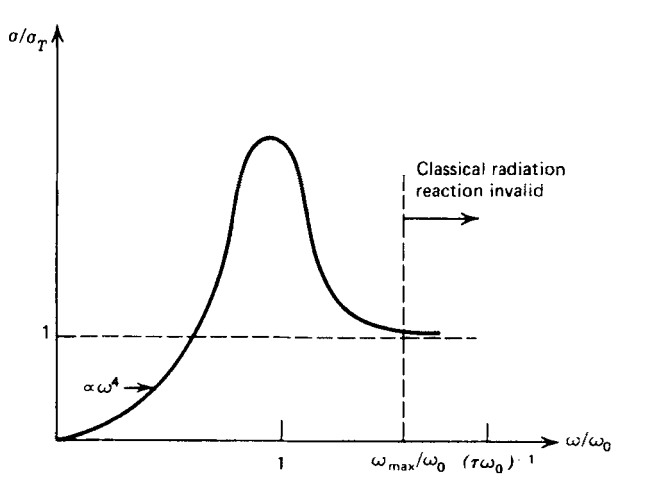
\includegraphics[width=0.8\textwidth]{img/ScatteringRayleigh}
\caption{Scattering di Rayleigh. Andamento della sezione d'urto in unità della sezione d'urto di Thomson in funzione della frequenza in unità di $\omega_0$.} \label{fig:Rayleigh}
\end{center}
\end{figure}

Lo scattering di Rayleigh della componente blu della luce solare da parte delle molecole dell'aria è il motivo principale per cui il cielo appare di colore azzurro, a causa della forte dipendenza della sezione d'urto dalla frequenza ($\propto\omega^4$). La radiazione ad alte frequenze ha una sezione d'urto maggiore di quella a basse frequenze, e pertanto viene diffusa più facilmente. Affinchè si abbia scattering Rayleigh, l'energia della radiazione deve essere inferiore all'energia di legame dell'elettrone col nucleo. Considerato che i principali componenti dell'atmosfera sono $\mathrm{N}_2$ e $\mathrm{O}_2$ (rispettivamente il $78 \%$ e il $21\%$) con energia di dissociazione pari rispettivamente a $9.39\, \mathrm{eV}$ e $5.15 \, \mathrm{eV}$, corrispondenti a fotoni di frequenza $\nu=2376 \, \mathrm{THz}$ e $\nu=1245 \, \mathrm{THz}$, (la luce rossa ha frequenza $\nu=428 \, \mathrm{THz}$, mentre quella blu $\nu=749 \, \mathrm{THz}$), la luce visibile è in grado di fare scattering Rayleigh nell'atmosfera: le componenti blu vengono scatterate facendo apparire il cielo blu, mentre le rimanenti gialle no, e vengono viste solo in direzione del sole.

\section[Bremsstrahlung]{Bremsstrahlung\footnote{Si pronuncia Bremstràlun.}}
In generale la bremsstrahlung è un qualsiasi tipo di radiazione dovuta all'accelerazione subita da una particella carica, compresa la radiazione di sincrotrone, di ciclotrone, e l'emissione di elettroni e positroni nel decadimento beta. Tuttavia questo termine viene comunemente usato per indicare la radiazione emessa da un elettrone libero nella materia, in seguito all'accelerazione provocata dall'interazione coulombiana con uno ione. Spesso ci si riferisce alla bremsstrahlung emessa da una plasma con il termine di radiazione free-free, per il fatto che in questo caso le cariche interagenti (elettrone e ione che genera il campo coulombiano che interagisce con l'elettrone) sono libere, o per lo meno, non legate tra loro sia prima che dopo l'interazione.
In generale questo processo va studiato con un approccio quantistico poichè possono essere prodotti fotoni di energie comparabili a quelle della particella emittente. Tuttavia un approccio classico, sotto opportune ipotesi, permette di giungere a conclusioni corrette, a cui vengono successivamente agggiunti gli effetti quantistici. Seguiremo quindi questo approccio più semplice, e trascureremo gli effetti relativistici, in quanto studieremo elettroni a temperature non superiori a $T=10^9\uK{}$. 

Iniziamo notando che la bremsstrahlung di due particelle identiche è nulla perchè in questo caso il momento di dipolo $\sum q_i \V{r}_i$  è semplicemente proporzionale al centro di massa del sistema $\sum m_i \V{r}_i$, che è una costante del moto, e quindi l'elemento di matrice associato alla transizione associata all'emissione, è nullo (poichè lo stato iniziale e lo stato finale sono diversi tra loro, e quindi ortogonali). Pertanto le particele devono essere diverse, ipotizziamo un elettrone e un generico ione di carica $Zq$. La particella emittente è l'elettrone in quanto più leggero e quindi subente un'accelerazione maggiore dello ione di massa $M$. A causa di ciò possiamo considerare un sistema di riferimento in cui lo ione è fermo, e resta tale per tutta l'interazione, e l'elettrone si avvicina su una traiettoria rettilinea lungo $\vers{x}$ a velocità $v\ll c$, traiettoria che ha distanza minima dallo ione pari a $b$, noto come \textit{parametro d'impatto}. Questo processo non è altro che lo scattering di Rutherford. Assumiamo che l'angolo di scattering $\phi \approx 0$, e calcoliamo la variazione di velocità in direzione $\vers{y}$ ortogonale alla direzione iniziale dell'elettrone. Ipotizziamo che il moto lungo $\vers{x}$ resti imperturbato, e quindi che $\V{v}_\mathrm{i} = (v,\,0)$, e $\V{v}_\mathrm{f} = (v,\,\Delta v)$. Indicando con $\V{r}$ il vettore che congiunge lo ione all'elettrone e con $\theta$ l'angolo tra $\V{r}$ e $\vers{x}$, abbiamo da semplici considerazioni geometriche che $\sin\theta = b/r$, e che $\tan\theta = b/x$, avendo fissato l'origine dell'asse $\vers{x}$ nel punto di minima distanza dallo ione. La forza che accelera l'elettrone in direzione $\vers{y}$ non è altro che la componente in tale direzione della forza coulombiana
\begin{equation}
F_y = -\dfrac{q^2Z}{r^2}\sin\theta = - \dfrac{q^2Z}{b^2}\sin^3\theta 
\end{equation}
Possiamo ora calcolare la variazione di velocità
\begin{align}
\Delta v &=  \int_{-\infty}^{+\infty} \dfrac{F_y}{m} \dd t = \int_{-\infty}^{+\infty} \dfrac{F_y}{m} \dfrac{\dd x}{v} = -\int_{0}^{\pi} \dfrac{F_y}{m} \dfrac{b}{\sin^2\theta}\, \dd \theta = \dfrac{2 q^2 Z}{m v b} \label{eq:Bremss3}
\end{align}
da cui vediamo subito che l'ipotesi che la variazione di velocità si piccola, $\Delta v \ll v$ equivale a 
\begin{equation}
\dfrac{q^2 Z}{b} \ll \inv{2}mv^2 \label{eq:Bremss6}
\end{equation}
cioè che l'energia cinetica dell'elettrone deve essere molto più grande dell'energia coulombiana massima, cioè quella raggiunta alla distanza minima elettrone-ione.
In media un elettrone in moto in un plasma subisce un gran numero di deflessioni, in direzioni tutte egualmente probabili, pertanto mediamente l'elettrone prosegue su traiettoria rettilinea, ovvero $\Delta v$ ha media nulla. Ciò non vale invece per $\Delta v^2$; data $n$ densità numerica degli ioni, il flusso di ioni visto dall'elettrone è $n\V{v}$. L'area di interazione con ciascuno ione è l'anello $2\pi\,b\,\dd b$. Pertanto la variazione temporale della quantità $\Delta v^2$ è data da $\Delta v^2$ per le interazioni per unità di tempo, integrata sul numero totale delle interazioni.
\begin{equation}
\der{}{t}(\Delta v)^2 = \int_{b_\mathrm{min}}^{b_\mathrm{max}} \left( \dfrac{2 q^2 Z}{m v b} \right)^2 nv\, 2\pi\,b\,\dd b = \dfrac{8\pi \,q^4 Z^2 n}{m^2 v} \ln \Lambda \label{eq:Bremss1}
\end{equation}
dove abbiamo definito 
\begin{equation}
\ln \Lambda \equiv \int_{b_\mathrm{min}}^{b_\mathrm{max}} \dfrac{\dd b}{b}
\end{equation}
noto come logaritmo coulombiano. Quando la \ref{eq:Bremss1} è dell'ordine di $v^2/\tau = v^3/ \mfp$, dove con $\tau$ si indica il tempo trascorso il quale la variazione di $v^2$ è dell'ordine della $v^2$ iniziale, mentre $\mfp$ indica il cammino libero medio, allora possiamo ricavare 
\begin{equation}
\mfp =\left(\inv{2}mv^2\right)^2 \inv{2\pi Z^2 q^4} \inv{n} \inv{\ln \Lambda} \approx \dfrac{(kT)^2}{2\pi Z^2 q^4} \inv{n} \inv{\ln \Lambda}
\end{equation}
dove nell'ultimo passaggio abbiamo approssimato l'energia cinetica all'energia termica.
Alcuni esempi sono il centro del sole in cui si ha $n\approx10^{26}\um{c}^{-3}$, $T\approx 10^7\uK{}$ che implica $\mfp \approx 10^{-8}\um{c}$, mentre per il vento solare si ha si ha $n\approx10^{-3}\um{c}^{-3}$, $T\approx 10^5\uK{}$ che implica $\mfp \approx 5\cdot 10^{13}\um{c}$, che è dell'ordine della distanza Terra-Sole $1 \uAU{} = 1.5\cdot 10^{13}\um{c}$.

A questo punto possiamo studiare lo spettro associato alla bremsstrahlung ricorrendo all'equazione \ref{eq:Larmor4}. Iniziamo studiando il quadrato della derivata seconda del momento di dipolo $\V{\ddot{d}}= -q\V{\dot{v}}$. Calcolando la trasformata di Fourier di questa relazione, otteniamo\footnote{Il primo membro deriva dal fatto che possiamo scrivere il momento di dipolo in termini della sua trasformata di Fourier
\begin{align*}
\V{\ddot{d}} = \dern{}{t}{2} \V{d}(t) = \dern{}{t}{2} \int_{-\infty}^{+\infty} \V{\tilde{d}}(\omega) e^{-i\omega t} \, \dd \omega = -\int_{-\infty}^{+\infty} \omega^2\V{\tilde{d}}(\omega) e^{-i\omega t} \, \dd \omega 
\end{align*} 
Notiamo che l'ultimo membro è l'antitrasformata della quantità $-\omega^2\V{\tilde{d}}(\omega)$. Pertanto risulta che la trasformata di Fourier di $\V{\ddot{d}}$ è $-\omega^2\V{\tilde{d}}(\omega)$, in quanto vale la proprietà $F\{ F^{-1}a(t)\} = a(t)$.}
\begin{equation}
-\omega^2 \tilde{\V{d}} = - \dfrac{q}{2\pi} \int_{-\infty}^{+\infty} \V{\dot{v}} e^{i\omega t} \, \dd t \label{eq:Bremss2}
\end{equation} 
Da questa relazione possiamo ottenere i valori di $\tilde{\V{d}}$ nei limiti di alte e basse frequenze. Anzitutto notiamo che l'interazione tra elettrone e ione ha una durata finita; assumendo che l'interazione avviene alla distanza $b$ tra le due particelle, il tempo di interazione, chiamato \textit{tempo di collisione} è dell'ordine di $\tau=b/v$. Per alte frequenze ($\omega\tau\gg 1$) l'esponenziale della \ref{eq:Bremss2} oscilla rapidamente, e l'integrale è piccolo; nel caso delle basse frequenze ($\omega\tau\ll 1$) l'esponenziale è essenzialmente unitario, e l'integrale vale quindi $\Delta v$. In altre parole si ha
\begin{align}
\omega^2 \V{\tilde{d}}(\omega) = 
\begin{cases}
\dfrac{q}{2\pi} \Delta\V{v} \,\,\,\,\,\,\,\,\,\,\,\,\,\,\,\,\,\,\,\, \omega\tau \ll 1 \\[10pt]
0 \,\,\,\,\,\,\,\,\,\,\,\,\,\,\,\,\,\,\,\,\,\,\,\,\,\,\,\,\,\,\,\,\,\, \omega\tau \gg 1 
\end{cases} \label{eq:Bremss4}
\end{align}
Possiamo ora sostituire la \ref{eq:Bremss3} nella \ref{eq:Bremss4} e quest'ultima nella formula di Larmor \ref{eq:Larmor4}, ottenendo
\begin{align}
\der{W}{\omega} = 
\begin{cases}
\dfrac{8\,Z^2 \,q^6}{3\pi \,c^3 \, m^2 \, v^2 \,b^2} \,\,\,\,\,\,\,\,\,\,\,\,\,\,\,\,\,\,\,\, \omega\tau \ll 1 \\[10pt]
0 \,\,\,\,\,\,\,\,\,\,\,\,\,\,\,\,\,\,\,\,\,\,\,\,\,\,\,\,\,\,\,\,\,\,\,\,\,\,\,\,\,\,\,\,\,\,\,\,\,\,\,\, \omega\tau \gg 1 
\end{cases} \label{eq:Bremss5}
\end{align}
Vediamo quindi che, dalla relazione tra tempo di collisione e parametro d'impatto, si ha emissione per $\omega b \ll v$, e quindi a parametri d'impatto piccoli corrispondono alte frequenze di emissione, e viceversa.

La discussione fatta finora tratta l'emissione da un singolo elettrone; determiniamo ora lo spettro totale per un mezzo con densità numerica di ioni $n_\mathrm{i}$ e densità numerica di elettroni $n_\mathrm{e}$. Il flusso di elettroni (numero di elettroni incidenti sull'unità di superficie nell'unità di tempo) è semplicemente $n_\mathrm{e}\,v$, e l'area di interazione tra elettroni e un singolo ione è $2\pi \, b\, \dd b$. La potenza emessa per unità di frequenza e di volume sarà quindi
\begin{equation}
\dfrac{\dd W}{\dd \omega\,\dd V \, \dd t} = n_\mathrm{e} n_\mathrm{i} \int_{b_\mathrm{min}}^{b_\mathrm{max}} v\, 2\pi \, b \der{W}{\omega} \, \dd b
\end{equation}
con $\der{W}{\omega}$ è dato dalla \ref{eq:Bremss5}. Sostituendo tale termine si trova facilmente
\begin{equation}
\dfrac{\dd W}{\dd \omega\,\dd V \, \dd t} = \dfrac{16}{3} \, \dfrac{n_\mathrm{e} n_\mathrm{i} \, Z^2\, q^6}{c^3\,m^2\,v} \, \ln\left(\dfrac{b_\mathrm{max}}{b_\mathrm{min}}\right) \label{eq:Bremss7}
\end{equation}
Dalla \ref{eq:Bremss5} vediamo che il valore limite del parametro d'impatto oltre il quale $\dfrac{\dd W}{\dd \omega}$ si annulla è $b_\mathrm{max} = v/\omega$. Il valore di $b_\mathrm{min}$ può invece essere stimato in due modi. Il primo considera il valore del parametro d'impatto a cui l'approssimazione di piccoli angoli di scattering non è più valida. Come visto precedentemente, questa condizione equivale alla \ref{eq:Bremss6}, che permette quindi di dare la stima
\begin{equation}
b_\mathrm{min}^{(1)} = \dfrac{2\,Z\,q^2}{m\,v^2}
\end{equation}
Una seconda stima può essere ottenuta seguendo un approccio quantistico. Dal principio di indeterminazione abbiamo $\Delta x\, \Delta p \gtrsim \hbar$, e prendendo $\Delta x \sim b$ e $\Delta p \sim mv$ otteniamo la seconda stima del parametro d'impatto
\begin{equation}
b_\mathrm{min}^{(2)} = \dfrac{\hbar}{mv}
\end{equation}
Quando $b_\mathrm{min}^{(1)} \gg b_\mathrm{min}^{(2)}$, equivalente alla condizione $\frac{1}{2} mv^2 \ll Z^2 \, Ry$\footnote{La quantità $Ry$ è l'energia di Rydberg per l'atomo di idrogno, definita come
\begin{align*}
Ry= \dfrac{m\, q^4}{2\hbar}
\end{align*}}
è possibile usare una descrizione classica del processo di scattering e utilizzare la \ref{eq:Bremss7}, con $b_\mathrm{min}^{(1)}$. Se invece vale $b_\mathrm{min}^{(1)} \ll b_\mathrm{min}^{(2)}$ il principio di indeterminazione svolge un ruolo importante e l'uso della \ref{eq:Bremss7}, con $b_\mathrm{min}^{(2)}$ è impreciso, anche se fornisce gli ordini di grandezza corretti. Per tutti i regimi il risultato esatto è espresso in termini del \textit{fattore di Gaunt} $g_\mathrm{ff}$ (il pedice indica free-free)
\begin{EQ}
\begin{equation}
g_\mathrm{ff} = \dfrac{\sqrt{3}}{\pi} \, \ln\left(\dfrac{b_\mathrm{max}}{b_\mathrm{min}}\right) 
\end{equation} 
\end{EQ}
in termini del quale la \ref{eq:Bremss7} diventa
\begin{EQ}
\begin{equation}
\dfrac{\dd W}{\dd \omega\,\dd V \, \dd t} = \dfrac{16\pi}{3\sqrt{3}} \, \dfrac{n_\mathrm{e} n_\mathrm{i} \, Z^2\, q^6}{c^3\,m^2\,v} \, g_\mathrm{ff} \label{eq:Bremss8}
\end{equation}
\end{EQ}
Sottolineiamo il fatto che in questa relazione la dipendenza dalla frequenza dell'emissione (e della velocità della particella) è contenuta nel fattore di Gaunt che a sua volta dipende dal parametro d'impatto.

\subsection{Bremsstrahlung termica}
Un'interessante applicazione delle formule appena ottenute è la loro applicazione alla bremsstrahlung termica, ovvero bremsstrahlung associata a particelle con velocità che seguono la \textit{distribuzione di Maxwell delle velocità}
\begin{EQ}
\begin{equation}
f(v, \,T) = 4\pi \left( \dfrac{m}{2\pi\,kT} \right)^{3/2}\, v^2\, \exp\left[-\dfrac{m\,v^2}{2\, kT}\right]
\end{equation}
\end{EQ}
Definiamo il coefficiente di emissione come l'energia emessa per unità di tempo, frequenza, angolo solido e volume\footnote{Il coefficiente di emissione quantifica la potenza emessa da un certo volume, in un certo intervallo infinitesimo di frequenze, entro un certo angolo solido.}
\begin{EQ}
\begin{equation}
j_\nu \equiv \dfrac{\dd W}{\dd t\, \dd \nu\, \dd V \, \dd\Omega} = \dfrac{2\pi}{4\pi} \dfrac{\dd W}{\dd t\, \dd \omega\, \dd V}
\end{equation}
\end{EQ}
dove la seconda riscrittura è esplicata in termini della quantità che compare nella \ref{eq:Bremss8}; in questo modo possiamo scrivere il coefficiente di emissione associato alla bremsstrahlung. Possiamo studiare l'emissione totale integrando su tutte le possibili velocità delle particelle: l'estremo di integrazione superiore è $+\infty$ poichè non si ha un limite superiore alle velocità delle particella, mentre l'estremo inferiore può essere ricavato introducendo effetti quantistici. I fotoni sono emessi con energia $h\nu$, quindi l'elettrone che li genera deve avere energia cinetica pari ad almeno questa quantità, quindi l'estremo inferiore è dato da
\begin{equation}
\inv{2} mv_\mathrm{min}^2 = h\nu
\end{equation}
Il valor medio del coeffieciente di emissione di bremsstrahlung termica è
\begin{equation}
j_\nu = \dfrac{\bigintsss_{v_\mathrm{min}}^{+\infty} {\frac{1}{2} \frac{\dd W}{\dd t\, \dd \omega\, \dd V} f(v, \,T) \, \dd v}}{{\int_{0}^{+\infty}  {f(v, \,T)}\, \dd v}} = \dfrac{8}{3}\, \dfrac{Z^2\, q^6}{m\,c^3} \left( \dfrac{2\pi}{3m\,kT} \right)^{1/2} \,n_\mathrm{e}\,n_\mathrm{i} \, e^{-h\nu/kT} \, \bar{g}_\mathrm{ff}
\end{equation}
dove $\bar{g}_\mathrm{ff}$ è il fattore di Gaunt mediato sulle velocità. Se chiamiamo $u \equiv h\nu/kT$ si ha che per $u\gg 1$ i valori di $\bar{g}_\mathrm{ff}$ non sono importanti in quanto lo spettro si annulla esmponenzialmente per tali valori di $u$. Se $u\approx 1$ allora $\bar{g}_\mathrm{ff}$ è dell'ordine dell'unità, mentre varia tra $1$ e $5$ per $10^{-4}<u<1$. 
\begin{figure}
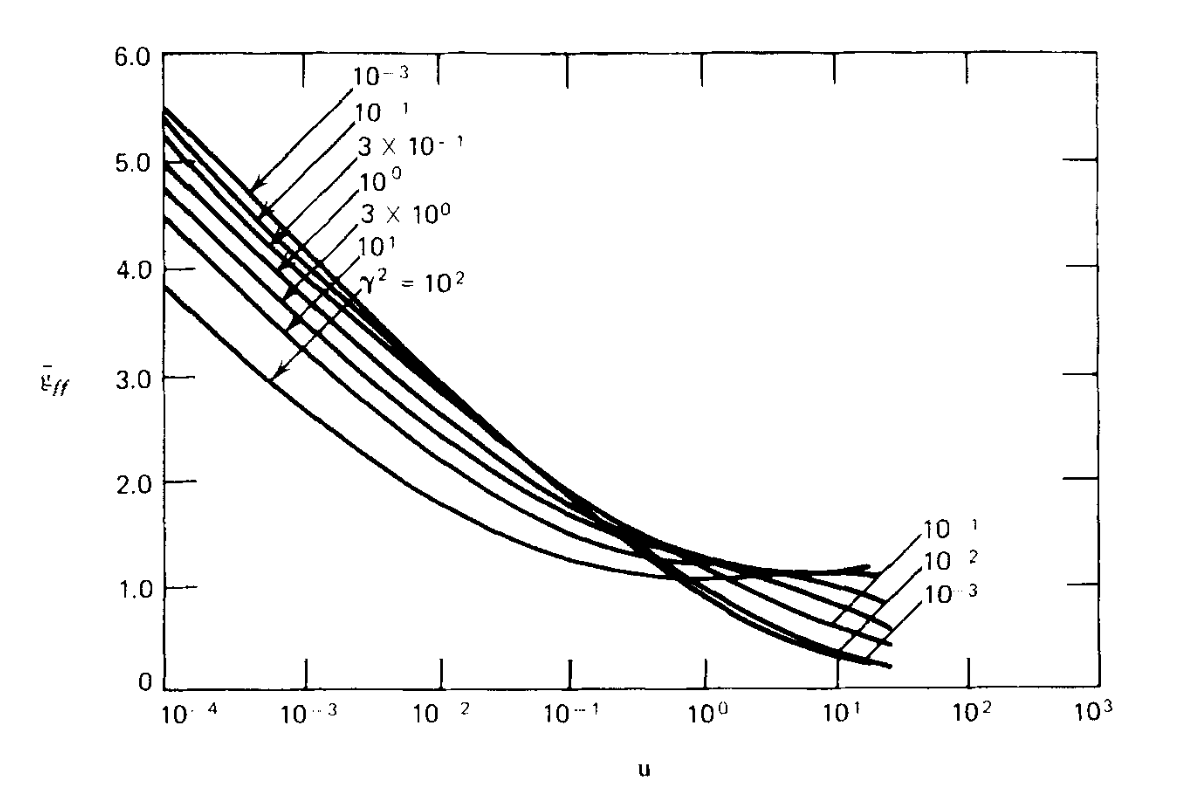
\includegraphics[width=0.8\textwidth]{img/Gaunt}
\caption{Andamento del fattore di Gaunt medio in funzione della quantità $u \equiv h\nu/kT$.} \label{fig:Gaunt}
\end{figure}
Notiamo infine che la dipendenza esponenziale di $j_\nu$ dalla frequenza $\nu$ implica che in un grafico log-log lo spettro è piuttosto piatto, fino al cutoff a circa $h\nu \approx kT$.\footnote{Questo è vero solo per un mezzo otticamente sottile, o trasparente. Non abbiamo infatti ancora considerato l'assorbimento dei fotoni da parte degli elettroni liberi che abbiamo finora considerato come dei semplici emettitori che non interagiscono più con la radiazione una volta emessa.} Perciò aumentando la temperatura il cutoff si sposta ad alte frequenze, e il plateau dello spettro si abbassa, a causa della dipendenza $j_\nu \propto T^{-1/2}$. Notiamo infine che integrando su tutte le frequenze si ottiene che \footnote{Essendo un plasma globalmente neutro si può approssimare $n_\mathrm{e}\,n_\mathrm{i} \approx n^2$ con $n$ densità numerica delle particelle del plasma.}
\begin{equation}
j = \int_0^{+\infty} j_\nu \, \dd \nu \propto n^2\, T^{1/2}
\end{equation}
che comporta che un plasma perde più facilmente energia tramite interazioni free-free quanto più grandi sono la temperatura e la densità.

L'emissione di bremsstrahlung consente di avere informazioni sulla densità e sulla temperatura del plasma negli ammassi di galassie, tramite la misurazione degli spettri nella banda X; il mezzo intracluster, a temperature tipiche di $10^7-10^8\uK{}$, ha come emissione principale quella di bremsstrahlung. Si può inoltre stimare che la radiazione di bremsstrahlung viene persa in tempi relativamente brevi, cioè il plasma raffredda velocemente. Perdendo energia termica non riesce più a mantenere l'equilibrio idrostatico e quindi collassa gravitazionalmente. Ciò non accade sempre in quanto in alcuni casi il plasma freddo viene mantenuto in equilibrio da altri processi.


\section{Trasporto radiativo}
Iniziamo col considerare un elemento di area $dA$ esposto ad una radiazione per un tempo $dt$. Definiamo il flusso di energia attraverso l'elemento di superficie come 
\begin{equation}
F=\frac{dE}{dA dt} \, ,
\label{eq:flusso}
\end{equation}
dove $dE$ è l'energia totale trasportata dalla radiazione %(cioè portata da raggi di tutte le frequenze dello spettro elettromagnetico) 
che attraversa l'elemento di area $dA$ nel tempo $dt$. Il flusso $F$ si misura in $\mathrm{erg\,s^{-1}\,cm^{-2}}$. Consideriamo ora l'elemento $dA$ orientato ortogonalmente ad un raggio di riferimento, e consideriamo tutti i raggi passanti per $dA$ la cui direzione è sottesa ad un angolo solido $d\Omega$ definito dal raggio di riferimento. L'energia che attraversa $dA$ in un tempo $dt$ e in un range di frequenze $d\nu$ è data da
\begin{equation}
dE=I_{\nu}\,dA\,dt\,d\Omega\,d\nu \, .
\label{eq:brillanza}
\end{equation}
Ques'equazione definisce l'intensità specifica o brillanza $I_{\nu}$, misurata in $\mathrm{erg\,s^{-1}\,cm^{-2}\,sr^{-1}\,Hz^{-1}}$. Se ipotizziamo ora di avere  $dA$ orientata arbitrariamente lungo la direzione $\textbf{n}$, si ha che il flusso differenziale attraverso l'elemento di superficie dovuto alla radiazione proveniente dall'angolo solido $d\Omega$ è 
\begin{equation}
dF_{\nu}=I_{\nu}\,cos{\theta}\,d\Omega\, ,
\label{eq:dflusso}
\end{equation}
dove $\theta$ è l'angolo compreso tra la direzione $\textbf{n}$ e la direzione del raggio che definisce $d\Omega$. Pertanto il flusso totale attraverso $dA$ è 
\begin{equation}
F_{\nu}=\int{I_{\nu}\,cos{\theta}\,d\Omega}\, .
\label{eq:Fintegrale}
\end{equation}
$F_{\nu}$ viene chiamato flusso monocromatico o specifico, misurato in Jy~\footnote{$1\, \mathrm{Jy} = 10^{-23}\,\mathrm{erg}\,\mathrm{s}^{-1}\,\mathrm{cm}^{-2}\,\mathrm{Hz}^{-1}$}, e integrandolo su tutte le frequenze permette di ottenere il flusso totale dell'equazione~\ref{eq:flusso}. 

La brillanza è da interpretarsi come una proprietà di un raggio luminoso (o meglio, di un fascio nell'angolo solido infinitesimo $\dd\Omega$); se non vi è materiale interposto nel tragitto di rpopagazione del raggio, si ha la conservazione della sua brillanza. Per dimostrarlo consideriamo oltre all'area $\dd A$, l'area infinitesima centrate nel punto $P$ distante $R$ da $\dd A$, e orientata in direzione $-\vers{n}$. Il flusso nella superficie in $P$ è $F_\nu = L_\nu /4\pi R^2$, mentre la brillanza in $P$ è data dal flusso in $P$ diviso l'angolo solido di provenienza del fascio, ovvero $\dd \Omega = \dd A /R^2$. QUindi risulta che $I_\nu = L_\nu /4\pi \dd A$, che implica che la brillanza lungo la direzione di propagazione si conserva (la sua derivata rispetto a $R$ è nulla) poichè dipende solo dalla potenza specifica emessa $L_\nu$\footnote{Si usa la $L$ perchè la potenza emessa è spesso indicata come luminiosità.} e dall'area emitente $\dd A$. 

\begin{Example}{Sfera di brilanza costante}
Supponiamo di avere una sfera di raggio $R$ e di brillanza costante $I_\nu = B$; qual è il flusso nel punto $P$ a distanza $r$ dal centro della sfera? Indichiamo con $\theta$ l'angolo compreso tra $r$ e la direzione congiungente il punto $P$ con un punto della superfiecie della sfera. Definiamo $\theta_\mathrm{c}$ l'angolo che definisce il cono d'ombra sulla superficie della sfera dal punto $P$, come mostrato nella figura \ref{fig:Sfera}. Risulta che l'intensità specifica in $P$ è $B$ se il raggio luminoso interseca la sfera, e nulla altrimenti.
Risulta allora che 
\begin{align*}
F_\nu = \int I_\nu \,\cos \theta \,\dd \Omega = B \int_{0}^{2\pi} \dd \phi \int_{0}^{\theta\mathrm{c}} \sin\theta \cos\theta \dd \theta = \pi\, B \, \sin^2\theta_\mathrm{c} = \pi B \dfrac{R^2}{r^2}
\end{align*}
Vediamo che ponend $r=R$, cioè considerando un punto della superficie, si ha che $F_\nu=\pi B$, quindi il flusso sulla superficie di una stella è pari a $\pi$ volte la sua brillanza.
\end{Example}
\begin{figure}
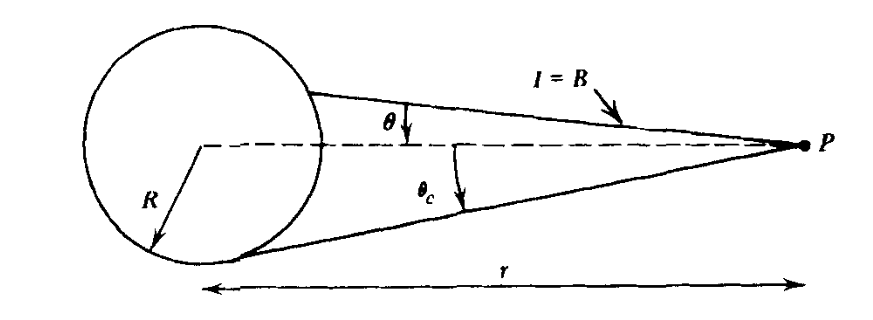
\includegraphics[width=\textwidth]{img/Brillanza_Sfera}
\caption{Schema di una sfera di brillanza costante $B$.} \label{fig:Sfera}
\end{figure}

Dopo aver definito queste grandezze possiamo considerare i due processi che alterano l'energia della radiazione in transito in un mezzo materiale: l'emissione e l'assorbimento.

\subsection{Emissione}

Si definisce coefficiente di emissione spontanea monocromatica $j_{\nu}$ l'energia emessa per unità di tempo, angolo solido, volume e frequenza:
\begin{equation}
dE=j_{\nu}\,dV\,d\Omega\,dt\,d\nu.
\label{eq:j}
\end{equation}
In generale il coefficiente $j_\nu$ dipende dalla direzione in cui avviene l'emissione. Nel caso in cui essa sia isotropa o nel caso di più emettitori distribuiti casualmente si può scrivere 
\begin{equation}
j_{\nu}=\frac{P_{\nu}}{4\pi},
\label{eq:jisotropico}
\end{equation}
dove $P_{\nu}$ è la potenza emessa per unità di volume e di frequenza. Per caratterizzare le emissioni spontanee viene utilizzata l'emissività $\epsilon_{\nu}$, definita come l'energia emessa spontaneamente su tutto l'angolo solido per unità di frequenza, tempo e massa:
\begin{equation}
dE=\epsilon_{\nu}\,\rho\,dV\,dt\,d\nu\,\frac{d\Omega}{4\pi},
\label{eq:emissività}
\end{equation}
dove $\rho$ indica la densità del mezzo emittente. Confrontando le equazioni \ref{eq:j} e \ref{eq:emissività} si ottiene una relazione tra emissività e coefficiente di emissione
\begin{equation}
j_{\nu}=\frac{\epsilon_{\nu}\rho}{4\pi},
\label{jepsilon}
\end{equation}
valida per un'emissione isotropa. Se si considera un fascio di sezione $dA$ che attraversa del materiale per un tratto $ds$, la variazione dell'intensità specifica del fascio dovuta all'emissione spontanea del mezzo è data da
\begin{equation}
dI_{\nu}=j_{\nu}\,ds.
\label{dIj}
\end{equation}

\subsection{Assorbimento}
Si definisce il coefficiente di assorbimento $\alpha_{\nu}$ mediante la seguente equazione
\begin{equation}
dI_{\nu}=-\alpha_{\nu}\,I_{\nu}\,ds,
\label{eq:alphaempirica}
\end{equation}
che rappresenta la perdità di intensità di un fascio che attraversa un materiale per un tratto $ds$. Questa legge fenomenologica può essere compresa considerando il materiale come composto da particelle con densità numerica $n$, ciascuna con una sezione d'urto di assorbimento $\sigma_{\nu}$, misurata in $\mathrm{cm^2}$. Consideriamo un volume infinitesimo cilindrico di altezza $ds$ e base $dA$ su cui incide una radiazione sottesa all'angolo solido $d\Omega$. L'energia del fascio che viene assorbita dal mezzo è
\begin{equation}
-dI_{\nu}\,dA\,d\Omega\,dt\,d\nu=I_{\nu}\,(n\,\sigma_{\nu}\,dA\,ds)\,d\Omega\,dt\,d\nu,
\end{equation} 
dove il termine tra parentesi indica l'area totale di assorbimento dovuta alle particelle. Da questa equazione segue immediatamente che
\begin{equation}
dI_{\nu}=-n\,\sigma_{\nu}\,I_{\nu}\,ds,
\end{equation}
che confrontata con l'equazione~\ref{eq:alphaempirica} implica
\begin{equation}
\alpha_{\nu}=n\sigma_{\nu}.
\end{equation}
Un modo più conveniente di esprimere il coefficiente di assorbimento in termini di proprietà microscopiche del mezzo (cioè mediante la sezione d'urto di assorbimento) è
\begin{equation}
\alpha_{\nu}=\rho\,\kappa_{\nu},
\end{equation}
dove $\rho$ è la densità di massa e $\kappa_{\nu}$, che si misura in $\mathrm{cm^2\,g^{-1}}$, è il coefficiente di assorbimento di massa, anche noto con il nome di opacità. Notiamo che i processi di scattering possono essere considerati come dei processi di assorbimento in quanto riducono la radiazione nella direzione di propagazione. Dando questa interpretazione è possibile definire l'\textit{opacità Thomson} come 
\begin{equation}
k_\mathrm{T} = \dfrac{\sigma_\mathrm{T}}{\mpr}
\end{equation}



\subsection{Equazione del trasporto radiativo}
Possiamo ora considerare il generico caso di un fascio che attraversa un mezzo materiale subendo una variazione di intensità che dipende sia dall'assorbimento che dall'emissione del materiale. Tenendo conto delle equazioni \ref{dIj} e \ref{eq:alphaempirica} otteniamo l'equazione del trasporto radiativo
\begin{equation}
\frac{dI_{\nu}}{ds}=-\alpha_{\nu}\,I_{\nu}+j_{\nu}. 
\label{trasportoradiativo1}
\end{equation}
Un modo più conveniente per scrivere l'equazione del trasporto radiativo è in termini della profondità ottica $\tau_{\nu}$, definita di seguito sia in forma differenziale che integrale
\begin{align}
&d\tau_{\nu}=\alpha_{\nu}\,ds\, ,
&\tau_{\nu}(s)={\int_{s_{0}}^s}\alpha_{\nu}(s')\,ds'\, ,
\label{eq:profonditàottica}
\end{align}
dove $s_{0}$ è un punto arbitrario che stabilisce lo zero della scala della profondità ottica. Grazie a questo  parametro adimensionale vengono definiti due diversi mezzi materiali, quelli otticamente spessi o opachi caratterizzati da $\tau_{\nu}>1$, e quelli otticamente sottili o trasparenti che hanno invece  $\tau_{\nu}<1$. Dividendo entrambi i membri dell'equazione \ref{trasportoradiativo1} per $\alpha_{\nu}$ si ottiene
\begin{equation}
\frac{dI_{\nu}}{d\tau_{\nu}}=-I_{\tau}+S_{\nu},
\label{trasportoradiativo2}
\end{equation} 
dove abbiamo definito la funzione sorgente $S_{\nu}$ come
\begin{equation}
S_{\nu}\equiv\frac{j_{\nu}}{\alpha_{\nu}}.
\end{equation}
Le soluzioni dell'equazione \ref{trasportoradiativo2} sono\footnote{
Per risolvere l'equazione moltiplichiamo l'equazione per un fattore $e^{\tau_\nu}$, e definiamo le quantità $\mathcal{I} \equiv I_\nu e^{\tau_\nu}$ e $\mathcal{S} \equiv S_\nu e^{\tau_\nu}$. In questo modo l'equazione diventa 
\begin{align*}
\der{\mathcal{I}}{\tau_\nu} = \mathcal{S}
\end{align*}
che ha soluzioni
\begin{align*}
\mathcal{I}(\tau_nu) = \mathcal{I}(0) + \int_0^{\tau_\nu}\mathcal{S}(\tau'_\nu )\, \dd \tau'_\nu
\end{align*}
Risostituendovi le definizioni di $\mathcal{I}$ e $\mathcal{S}$ si ottengono le soluzioni finali dell'equazione del trasporto radiativo.}
\begin{equation}
I_{\nu}(\tau_{\nu})=I_{\nu}(0)\,e^{-\tau_{\nu}}+\int_0^{\tau_{\nu}}e^{-(\tau_{\nu}-\tau_{\nu}')}\,S_{\nu}(\tau_{\nu}')\,d\tau_{\nu}'\,, \label{eq:soluzionitrasportoradiativo0}
\end{equation}
che viene facilmente interpretata come somma di due termini: l'intensità iniziale del fascio diminuita esponenzialmente dall'assorbimento, più la funzione sorgente del mezzo integrata e diminuita dall'assorbimento del mezzo stesso. Il significato della funzione sorgente appare più chiaro se si considera un mezzo con $S_{\nu}$ costante, cioè che non dipende dalla profondità ottica. In questo caso l'equazione \ref{eq:soluzionitrasportoradiativo0} si riduce a 
\begin{equation}
I_{\nu}(\tau_{\nu})=I_{\nu}(0)\,e^{-\tau_{\nu}}+S_{\nu}(1-e^{-\tau_{\nu}})\,,
\label{soluzionitrasportoradiativo}
\end{equation}
da cui segue immediatamente che $I_{\nu}{\rightarrow}S_{\nu}$ per $\tau_{\nu}\rightarrow\infty$. Osservando l'equazione \ref{trasportoradiativo2} si nota che se $I_{\nu}>S_{\nu}$ allora $\frac{dI_{\nu}}{d\tau_{\nu}}<0$ e $I_{\nu}$ tende a decrescere lungo la direzione di propagazione. Se invece $I_{\nu}<S_{\nu}$, $\frac{dI_{\nu}}{d\tau_{\nu}}>0$ e $I_{\nu}$ cresce lungo la direzione di propagazione. Questo risultato permette di dare un'interpretazione fisica della funzione sorgente come la quantità a cui tende l'intensità specifica di un fascio che attraversa un mezzo materiale, e che raggiunge per profondità ottiche sufficientemente grandi ($\tau_{\nu}\rightarrow\infty$).

Un modo equivalente di descrivere l'assorbimento è in termini del libero cammino medio. Questo è definito come la distanza media percorsa dai fotoni in un materiale, senza che questi vengano assorbiti. Abbiamo già incontrato questa grandezza parlando dello scattering: in generale è definita libero cammino medio la distanza media percorsa da una particella (in questo caso un fotone) senza interagire con un'altra particella (in questo caso gli elettroni del mezzo assorbente). Dalla relazione \ref{eq:alphaempirica} risulta che la probabilità di un fotono di viaggiare per almeno una profondità ottica $\tau_\nu$ è sempliciemente $e^{-\tau_\nu}$. La profondità ottica media è quindi pari all'unità\footnote{\begin{align*}
<\tau_\nu> \equiv \int_{0}^{+\infty} \tau_\nu e^{-\tau_\nu} \, \dd \tau_nu = 1
\end{align*}}
e questo permette di ricavare il libero cammino medio che corrisponde quindi al reciproco del coefficiente di assorbimento\footnote{Perchè vale $<\tau_nu>=\alpha_nu\lambda_\nu = 1$.}.


\section{Radiazione termica}
La radiazione termica è la radiazione emessa da materia all'equilibrio termico. Per studiare le proprietà di questa radiazione occorre prima studiare la \textit{radiazione di corpo nero}.

\subsection{Radiazione di corpo nero}
Consideriamo un sistema isolato termicamente a tamperatura $T$, e tale che la radiazione non possa nè entrare nè uscire. Ipotizziamo ora di praticare un piccolo forellino che permetta di misurare la radiazione interna senza perturbare l'equilibrio. Essendo i fotoni privi di massa, essi possono essere creati e distrutti in numeri arbitrari  all'interno del contenitore; non si ha quindi una conservazione del numero dei fotoni. 
Dimostriamo ora che $I_\nu$ è indipendente dalle proprietà del contenito e dipende solo dalla sua temperatura. Ipotizziamo di unire il contenitore con un altro con diversa forma ma alla stessa temperatura, e interporre tra i due forellini un filtro che consente il passaggio di una singola frequenza. Se fosse che $I_\nu \neq I'_\nu$ allora l'energia transità spontaneamente tra i due sistemi, ma questo è in disaccordo col secondo principio della termodinamica, poichè i due sistemi sono alla stessa temperatura. Risulta quindi che $I_\nu \equiv B_\nu(T)$, ovvero che l'intensità specifica è una funzione della sola temperatura del sistema. 

Consideriamo ora un elemento di materiale emettente alla temperatura $T$, in equilibrio termico, e poniamolo all'interno di una cavità di corpo nero alla stessa temperatura $T$. Se il materiale ha una funzione sorgente $S_\nu$ tale che $S_\nu>B_\nu$ allora $I\nu>B_\nu$, e se $S_\nu<B_\nu$ allora $I\nu<B_\nu$, per quanto la discussione dopo l'equazione \ref{soluzionitrasportoradiativo}. Tuttavia la presenza del materiale nella cavità di corpo nero non può alterare la radiazione poichè anche la nuova configurazione è un corpo nero alla stessa temperatra $T$ di quello iniziale. Pertanto abbiamo le reazioni
\begin{align}
S_\nu &= B_\nu(T) \\
j_\nu &= \alpha_\nu B_\nu(T) \label{eq:Kirchhoff}
\end{align}
dove l'ultima è nota come \textit{legge di Kirchhoff}, che afferma che per un corpo di un generico materiale che assorbe ed emette radiazione elettromagnetica in equilibrio termodinamico, il rapporto tra i coefficienti di emissione e di assorbimento, ovvero la funzione sorgente, è una funzione universale della frequenza della radiazione, e della temperatura del corpo. 
L'equazione del trasporto radiativo della radiazione termica diventa quindi
\begin{equation}
\der{I_\nu}{s} = -\alpha_\nu I_\nu + \alpha_\nu B_\nu(T)
\end{equation}
Possiamo ora fare una distinzione tra radiazione termica, in cui $S_\nu=B_\nu$ e radiazione di corpo nero in cui $I_\nu=B_\nu$. La radiazione termica diventa radiazione di corpo nero solo per mezzi otticamente spessi. Infatti la radiazione termica è la radiazione emessa da un mezzo in equilibrio termico; se poi il mezzo è anche in equilibrio con il campo di radiazione (condizione che richiede di essere otticamente spesso) allora si ha radiazione di corpo nero. In poche parole la radiazione è detta \textit{termica} se il mezzo emettente è solo in equilibrio termodinamico, mentre è detta di \textit{corpo nero} se è anche in equilibrio con il campo di radiazione elettromagnetica.

La funzione $B_{\nu}(T)$ è la brillanza di un corpo nero, e coincide con la funzione di Planck che viene di seguito definita in termini della frequenza e della lunghezza d'onda
\begin{align}
&B_{\nu}(T)=\frac{2\,h\,\nu^3}{c^2}\dfrac{1}{e^{{h\nu}/{k_\mathrm{B}\,T}}-1}\, ,
&B_{\lambda}(T)=\frac{2\,h\,c^2}{\lambda^5}\frac{1}{e^{{h\,c}/{\lambda\,k_\mathrm{B}\,T}}-1}\, ,
\end{align}
dove $h$, $c$, $k_\mathrm{B}$ sono rispettivamente la costante di Planck, la velocità della luce e la costante di Boltzmann. Grazie a questa funzione possiamo ottenere alcune utili proprietà del corpo nero (non le dimostreremo)

\begin{itemize}
\item{\textbf{Legge di Stefan-Boltzmann}} \begin{align}
F = \int_0^{\infty} F_\nu \, \dd \nu = \pi \int_0^\infty B_\nu \, \dd \nu = \sigma T^4
\end{align}
\item{\textbf{Legge di Rayleigh-Jeans}} Nel limite $h\nu \ll kT$ si ha
\begin{align}
B_\nu(T) \approx \dfrac{2\nu^2}{c^2}\, kT
\end{align}
\item{\textbf{Legge di Wien}} Nel limite $h\nu \gg kT$ si ha
\begin{align}
B_\nu (T) = \dfrac{2h\nu^3}{c^2} \, \exp{-\dfrac{h\nu}{kT}}
\end{align}
\item{\textbf{Legge dello spostamento di Wien}}
\begin{align}
T\, \lambda_max = b
\end{align}
dove $b$ è detta costante dello spostamento di Wien.
\end{itemize}
Nella figura \ref{fig:Planck} è riportato lo spettro di corpo nero.
\begin{figure}
\begin{center}
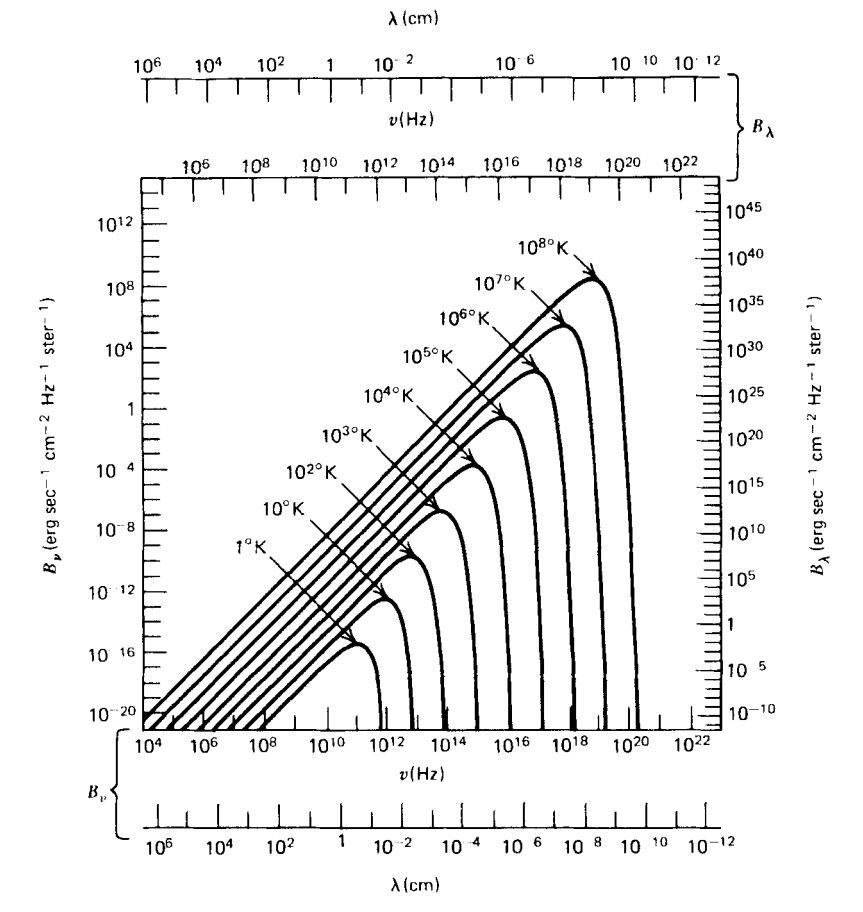
\includegraphics[width=0.8\textwidth]{img/Spettro_di_Planck}
\caption{Spettro della radiazione di corpo nero alle varie temperature.} \label{fig:Planck}
\end{center}
\end{figure}

Concludiamo definendo due quantità spesso utilizzate in astrofisica. La prima è la \textit{temperatura di brillanza} definita come la temperatura $T_\mathrm{B}$ a cui la brillanza di corpo nero assume lo stesso valore dell'intensità specifica osservata alla frequenza $\nu$, ovvero $I_\nu = B_\nu(T_\mathrm{B})$. Grazie a questa temperatura è possibile interscambiare la brillanza con la temperatura. Questa procedura viene spesso adottata in radioastronomia in cui è possibile applicare la legge di Rayleigh-Jeans. In questa approssimazione l'equazione del trasporto radiativo può essere espressa come
\begin{equation}
\der{T_\mathrm{B}}{\tau_\nu} = - T_\mathrm{B} + T \,\,\,\,\,\,\,\,\,\,\,\,\,\,\,\longrightarrow \,\,\,\,\,\,\,\,\,\,\,\,\,\,\ T_\mathrm{B} = T_\mathrm{B}(0)e^{-\tau_\nu} + T(1-e^{-\tau_\nu})
\end{equation}
con $T$ temperatura del materiale emettente. Questo implica che se il mezzo è otticamente spesso la temperatura del materiale tende alla temperatura di brillanza della radiazione. Notiamo infine che l'unicità della definizione della temperatura di brillanza in questo regime di basse frequenze dipende dalla monotonia della funziane di Rayleigh-Jenas. Inoltre in generale la temperatura di brillanza è funzione della frequenza; solo se la sorgente è un corpo nero la temperatura di brillanza è la stessa a tutte le frequenze.

L'altra quantità è la \textit{temperatura effettiva} $T_\mathrm{eff}$, definita come la temperatura a cui il flusso totale di corpo nero coincide con il suo flusso totale effettivo (misurato), cioè $F=\sigma T_\mathrm{eff}^4$.

\subsection{Coefficienti di Einstein}
La legge di Kischhoff lega il coefficienti di assorbimento e di emissione per un emettitore termico, relazione che deve necessariamente avere una spiegazione a livello microscopico. Tale legame fu scoperto studiato da Einstein tramite una semplice analisi dell'interazione tra la radiazione e un atomo. Seguendo il suo approccio, consideriamo due livelli energetici, il primo a energia $E$ e peso statistico $g_1$, mentre il secondo a energia $E+h\nu_0$ con peso statistico $g_2$. Durante l'assorbimento il sistema passa dallo stato 1 allo stato 2, con l'assorbimento di un fotone di energia $h\nu_0$, mentre nella transizione dallo stato 2 allo stato 1 si ha l'emissione di un fotone di energia $h\nu_0$. Distinguiamo 3 diversi processi:
\begin{itemize}
\item[1] \textbf{Emissione spontanea} Si ha emissione spontanea quando il sistema si trova nel livello 2 e decade nel livello 1 emettendo un foton, in assenza di un campo radiativo esterno. Definiamo il coefficiente di Einstein $A_{21}$ come la probabilità di transizione per unità di tempo di avere un'emissione spontanea.
\item[2] \textbf{Assorbimento} \\ Si ha assorbimento in presenza di un fotone di energia $h\nu_0$ che viene assorbito permettendo al sistema di passare dallo stato 1 allo stato 2. Ci aspettiamo che la probabilità per unità di tempo che accada questo processo sia proporzionale alla densità di fotoni emessi, o equivalentemente all'intensità specifica media alla frequenza di emissione $\nu_0$ ovvero
\begin{equation}
J_\nu = \inv{4\pi} \int_0^\infty I_\nu \, \dd \Omega \label{eq:Einstein4}
\end{equation} 
Per essere precisi la differenza di energia tra i due livelli non è associata unicamente a fotoni alla frequenza $\nu_0$, ma anche da fotoni a frequenza in un intorno di $\nu_0$. Indichiamo con $\phi(\nu)$ la funzione piccata in $\nu_0$ che descrive le frequenze associate alla transizione. L'intensità media associata all'assorbimento sarà 
\begin{equation}
 J \equiv \int_0^\infty J_\nu \phi (\nu) \, \dd \nu \label{eq:Einstein3}
\end{equation}
La probabilità per unità di tempo di assorbimento sarà proporzionale a $J$; definiamo la costante di proporzionalità come il coefficiente di Einstein $B_{12}$.
\item[2] \textbf{Emissione stimolata}  \\ Einstein scoprì che per derivare la legge di planck era necessario che un altro processo fosse proporzionale a $J$ e causasse l'emissione di un fotone. Tale processo è l'emissione stimolata, e il coefficiente di proporzionalità tra la probabilità per unità di tempo di emissione stimolata e $J$ è il coefficiente di Einstein $B_{21}$.
\end{itemize}
Troviamo ora le relazioni tra i coefficienti di Einstein. All'equilibrio termodinamico si ha che il numero di transizioni per unità di tempo e di volume dallo stato 1 allo stato 2 è uguale al numero di transizioni per unità di tempo e di volume dallo stato 2 allo stato 1. Pertanto, indicando con $n_1$ e $n_2$ rispettivamente le densità numeriche di atomi nello stato 1 e nello stato 2, la condizione di equilibrio termodinamico equivale a
\begin{equation}
n_1 B{12}J = n_2 A_{21} + n_2 B_{21} J \label{eq:Einstein2}
\end{equation}
che permette di ricavare $J$
\begin{equation}
J = \dfrac{A_{21}/B_{21}}{(n_1/n_2)(B_{12}/B_{21})-1} \label{eq:Einstein1}
\end{equation}
All'equilibrio termodinamico vale 
\begin{equation}
\dfrac{n_1}{n_2}=\dfrac{g_1 \exp[-E/kT]}{g_2 \exp[-(E+h\nu_0)/kT]} = \dfrac{g_1}{g_2}\exp[h\nu_0/kT]
\end{equation}
che può essere sostituita nella \ref{eq:Einstein1}. Essendo all'equilibrio termodinamico, $J_\nu=B_\nu$, e il vatto che $B_\nu$ varia lentamente sula scala di $\Delta\nu$ implica che anche $J=B_\nu$. Pertanto affinchè valga quest'ultima eguaglianza devono valere le relazioni
\begin{EQ}
\begin{align}
&g_1 B_{12} = g_2 B_{21}
&A_21 = \dfrac{2h\nu^3}{c^2} B_{21}
\end{align}
\end{EQ}
dette \textit{relazioni di Einstein}, e sono un esempio di \textit{relazioni di bilancio dettagliato} ovvero relazioni tra un processo microscopico e il suo inverso (assorbimento-emissione). Le relazioni di Einstein non dipendono dalla temperatura del sistema, quindi devono essere valide indipendentemente dal fatto che il sistema sia in equilibrio termodinamico e sono un'estensione della legge di Kirchhoff allo scopo di includere emissione non termica, che si manifesta quando la materia non è in equilibrio termodinamico. Se si riesce a determinare uno dei tre coefficienti, le relazioni di Einstein consentono di determinare gli altri due. Come abbiamo detto, il fatto che viene incluso il processo di emissione stimolata, serve a ottenere la legge di Planck (ciò apparirà più chiaro più avanti, nella discussione della legge di Kirchhoff generalizzata nel caso di equilibrio termico).

Resta ora da ricavare la relazione tra i coefficeinti di Einstein e i coefficienti di emissione e di assorbimento $j_\nu$ e $\alpha_\nu$. Per ottenere il primo assumiamo che la distribuzione delle frequenze della radiazione emessa durante un processo di emissione spontanea sia la stessa funzione $\phi(\nu)$ che descrive la distribuzione delle frequenze associate all'assorbimento. Per definizione, l'energia $E$ emessa in un volume $\dd V$, nel tempo $\dd t$, entro un angolo solido $\dd \Omega$, e in un range di frequenze $\dd \nu$ è $j_\nu\,\dd V\, \dd\Omega\,\dd\nu\,\dd t$. Poichè ciascun atomo contribuisce  con un'energia $h\nu_0$ distribuita su tutto l'angolo solido $4\pi$ per ciascuna transizione, si può esmpirmere l'energia $E$ come $(h\nu_0/4\pi)\,\phi(\nu)\,n_2\,A_{21}\,\dd V\, \dd\Omega\,\dd\nu\,\dd t$ e si ottiene cos' la relazione tra il coefficiente di emisisone e il coefficiente $A$ di Einstein
\begin{EQ}
\begin{equation}
j_\nu = \dfrac{h\nu_0}{4\pi}\,n_2\,A_{21}\,\phi(\nu)
\end{equation}
\end{EQ}
Per ottenere una relazione analoga per il coefficiente di assorbimento ricoridamo che la quantità $B_{12}J$ è la probabilità di transizione per unità di tempo associata all'assorbimento.Segue quindi che, sfruttando le definizioni \ref{eq:Einstein3} e \ref{eq:Einstein4}, si ha che l'energia totale assorbita nel tempo $\dd t$ dal volume $\dd V$ è 
\begin{align*}
\dd V\,\dd t \, h\nu_0\,n_1\,B_{12}\inv{4\pi} \int_0^{4\pi} \dd \Omega \int_0^\infty \phi(\nu)\,I_\nu \, \dd\nu
\end{align*}
Pertanto l'energia assorbita nel range di frequenze $\dd\nu$, proveniente dall'angolo solido $\dd\Omega$, nel tempo $\dd t$, dal volume $\dd V$ è 
\begin{align*}
\dd V\, \dd\Omega\,\dd\nu\,\dd t \dfrac{h\nu_0}{4\pi}\,n_1\,B_{12} \,\phi(\nu)\,I_\nu
\end{align*}
Tenendo conto dell'equazione \ref{eq:alphaempirica}  si ottiene
\begin{equation}
\alpha_\nu = \dfrac{h\nu_0}{4\pi} \, n_1\, B_{12}\,\phi(\nu) \label{eq:Einstein5}
\end{equation}
Questa non è la relazione finale tra coefficienti di Einstein  e di assorbimento, infatti non abbiamo considerato l'emissione stimolata. In quanto emissione si potrebbe pensare in un primo momento di aggiungere un fattore correttivo al coefficiente di emissione che tenga conto di questo processo. Tuttavia l'emissione stimolata è provocata dalla presenza di un campo radiativo esterno, al pari dei processi di assorbimento. Mentre si può avere emissione spontantea senza la presenza di radiazione esterna, non è possibile avere in tali condizioni nè emissione stimolata nè assorbimento. Pertanto si considera l'emissione stimolata come un assorbimento negativo, e si includono i suoi effetti nel coefficiente di assorbimento $\alpha_\nu$. Sfruttando lo stesso ragionamento usato per ottenere la \ref{eq:Einstein5}, si ottiene il contributo dovuto all'emissione stimolata. Il coefficiente di assorbimento è quindi legato ai coefficienti $B$ di Einstein dalla relazione
\begin{EQ}
\begin{equation}
\alpha_\nu = \dfrac{h\nu_0}{4\pi} (n_1\,B_{12}-n_2\,B_{21})\,\phi(\nu) \label{eq:Einstein7}
\end{equation}
\end{EQ}
Se ora calcoliamo il rapporto tra coefficiente di emissione e di assorbimento, possiamo esprimere la funzione sorgente come
\begin{EQ}
\begin{equation}
S_\nu = \dfrac{2h\nu^3}{c^2}\tonde{\dfrac{g_2n_1}{g_1n_2}}^{-1}
\end{equation}
\end{EQ}
equazione che prende il nome di \textit{legge di Kirchoff generalizzata}. Tre casi interessanti di questa equazione sono
\begin{itemize}
\item[1]\textbf{Emissione termica (LTE)} \\
Se la materia si trova in equilibrio termico con se stessa, ma non necessariamente con il campo radiativo, si ha
\begin{equation}
\dfrac{g_2n_1}{g_1n_2} = \exp\quadre{\dfrac{h\nu}{kT}} \label{eq:Einstein6}
\end{equation}
Il questo caso la materia viene detta in \textit{equilibrio termodinamico locale} (LTE).
Sostituendo nella legge di Kirchhoff generalizzata si ottiene quanto ci aspettiamo dalla legge di Kirchoff \ref{eq:Kirchhoff}, ovvero che la funzione sorgente coincide con la funzione di Planck. Se si trascurasse il processo di emissione stimolata, il coefficiente di assorbimento è dato dalla \ref{eq:Einstein5}. In questo caso, calcolando la funzione sorgente non si ottiene più la legge di Planck\footnote{La funzione sorgente è data dal rapporto $j_\nu/\alpha_\nu$, che viene calcolato usando le relazioni tra tali parametri e i coefficienti di Einstein. Sostituendovi poi la \ref{eq:Einstein6} si ottiene la funzione di Planck nel regime di Wien}, bensì la sua approssimazione nel regime di Wien. Non tenendo conto dei processi di emissione stimolata, si ottiene quindi un risultato errato, o meglio, non generale. L'approssimazione di Wien della legge di Planck è infatti valida solo in un certo range di frequenze, ovvero $h \nu \gg kT$. Questa condizione implica che il livello 2 è scarsamente popolato rispetto al livello 1 (poichè la separazione energetica $h\nu$ tra i livelli è molto più grande dell'energia termica del sistema), ovvero $n_2 \ll n_1$. Questo implica a sua volta dalla \ref{eq:Einstein7}, che l'emissione stimolata è trascurabile rispetto all'assorbimento, e quindi la funzione sorgente che si ottiene è la funzione di Planck nel regime di Wien. Pertanto, tenendo in considerazione il processo di emissione stimolata si ottiene una funzione sorgente pari alla funzione di Wien solo nel regime delle alte frequenze, mentre non tenendo in considerazione tale processo si ottiene la funzione di Wien a tutte le frequenze, risultato in contraddizione con la legge di Kirchhoff \ref{eq:Kirchhoff}.
\item[2]\textbf{Emissione non termica } \\
In questo caso sono compresi tutti i casi in cui
\begin{equation}
\dfrac{g_2n_1}{g_1n_2} \neq \exp\quadre{\dfrac{h\nu}{kT}} 
\end{equation}
Un esempio è un plasma in cui gli elettroni non seguono una distribuzione maxwelliana delle velocità.
\item[3]\textbf{Popolazioni invertite - Maser } \\
Questo è il caso in cui il sistema è in equilibrio termico e vale
\begin{equation}
\dfrac{n_2g_1}{n_1g_2} =  \exp\quadre{-\dfrac{h\nu}{kT}}  >1
\end{equation}
Tipicamente vale questa relazione ma con il segno $<$, equivalente a dire $n_1/g_1>n_2/g_2$, cioè il livello energetico inferiore è il più popolato. Nel caso di una \textit{popolazione invertita} si ha invece $n_1/g_1<n_2/g_2$, condizione che implica un coefficiente di assorbimento negativo ($\alpha_\nu<0$). Questo significa che anzichè perdere intensità attraversando il materiale, il fascio acquista energia. Un sistema del genere è detto \textit{maser} (microwave amplification by stimulater emission of radiation) l'equivalente nelle microonde del \textit{laser}. 
\end{itemize}

\section{Approssimazione di Rosseland}
In mezzi materiali come l'interno delle stelle si ha un altro grado di omogeneità locale che consente di relazionare il flusso di energia con il gradiente locale di temperatura. Questo risultato è noto con il nome di \textit{approssimazione di Rosseland}, che ricaveremo in questa sezione.

Facendo riferimento all'immagine \ref{fig:Rosseland} assumiamo che l'emissione termica osservata propaga per piani paralleli, cioè lungo una direzione privilegiata $\vers{z}$. Questa approssimazione viene spesso usata anche per le stelle, nel limite $z\ll R_\star$, di modo che si possa considerare questa simmetria anche per un sistema sferico. Indichiamo con $\vers{n}$ la direzione di osservazione, direzione che forma con l'asse $\vers{z}$ un angolo $\theta$. Per semplici considerazioni geometriche si ha
\begin{equation}
\dd s= \dfrac{\dd z}{\cos\theta}\equiv\dfrac{\dd z}{\mu}
\end{equation}
\begin{figure}
\begin{center}
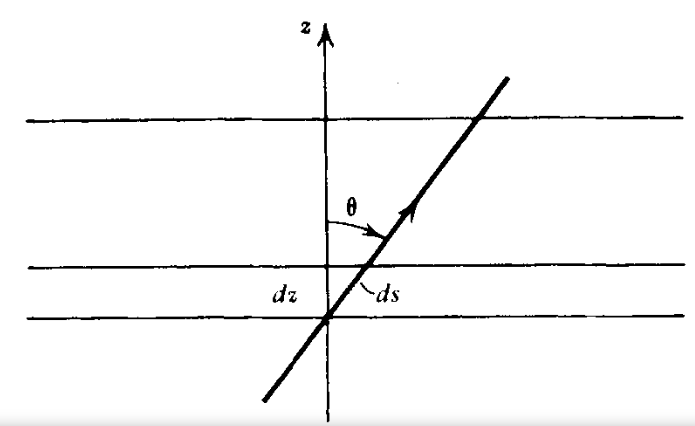
\includegraphics[width=0.8\textwidth]{img/Rosseland}
\caption{Approssimazione dei piani paralleli usata nell'approssimazione di Rosseland} \label{fig:Rosseland}
\end{center}
\end{figure}
Riscriviamo l'equazione del trasporto radiativo nella seguente forma
\begin{equation}
I_\nu = S_\nu - \inv{\alpha_\nu} \der{I_\nu}{s}
\end{equation}
con $S_\nu = B_\nu(T)$ poichè stiamo considerando radiazione termica. Se il coefficiente di assorbimento è grande, allora $I_\nu = S_\nu$, e quindi la brillanza coincide con la funzione di Planck. Quindi il flusso della \ref{eq:dflusso} è nullo poichè la funzione di Planck non dipende dagli angoli (è isotropa). Ricaviamo una stima all'ordine successsivo, ricordando che la stima all'ordine zero è $I_\nu^{(0)} = S_\nu$. Otteniamo
\begin{equation}
I_\nu^{(1)} = S_\nu - \inv{\alpha_\nu} \der{I_\nu}{s} = B_\nu(T) - \dfrac{\mu_\nu}{\alpha_\nu}\der{B_\nu}{z}
\end{equation}
Pertanto il flusso è 
\begin{equation}
F_\nu = 2\pi \, \int_{-1}^{+1} I_\nu^{(1)} \mu \, \dd \mu = - \dfrac{2\pi}{\alpha_\nu} \, \int_{-1}^{+1} \der{B_\nu(T)}{z} \, \mu^2 \,\dd\mu = -\dfrac{4\pi}{3} \inv{\alpha_\nu}\der{B_\nu(T)}{z}
\end{equation}
Abbiamo ottenuto un'espressione del flusso monocromatico in termini del gradiente della funzione di Planck. Per stimare il flusso totale consideriamo il fatto che la funzione di Planck dipende da $z$ tramite la temperatura, pertanto
\begin{equation}
\der{B_\nu}{z} = \der{B_\nu}{T}\der{T}{z}
\end{equation}
Possiamo ora calcolare il flusso totale integrando il flusso monocromatico su tutte le frequenze
\begin{equation}
F = \int_0^\infty F_\nu \, \dd \nu = -\dfrac{4\pi}{3} \der{T}{z} \int_0^\infty \inv{\alpha_\nu} \der{B_\nu}{T}\, \dd \nu
\end{equation}
Sfruttando il fatto che 
\begin{equation}
\int_0^\infty \der{B_\nu}{T}\, \dd \nu = \der{}{T} \int_0^\infty B_\nu\, \dd \nu = \der{}{T} \left(\dfrac{\sigma T^4}{\pi} \right) = \dfrac{4\sigma T^3}{\pi}
\end{equation}
e definendo il \textit{coeffieciente di assorbimento medio di Rosseland} come 
\begin{equation}
\inv{\alpha_\mathrm{R}} = \dfrac{\int_0^\infty \inv{\alpha_\nu} \der{B_\nu}{T}\, \dd \nu}{\int_0^\infty  \der{B_\nu}{T}\, \dd \nu}
\end{equation}
possiamo ottenere un'espressione del flusso totale dovuto a emissione termica, in termini del gradiente di temperatura del mezzo emittente
\begin{EQ}
\begin{equation}
F=-\dfrac{16}{3} \dfrac{\sigma T^3}{\alpha_\mathrm{R}} \der{T}{z} \label{eq:Rosseland1}
\end{equation}
\end{EQ}
Questa relazione è spesso chiamata \textit{equazione di diffusione radiativa}. Mostra che il trasporto radiativo dell'energia è dello stesso tipo della conduzione di calore, con una conduttività pari a $16\sigma T^3 / 3\alpha_\mathrm{R}$. Anche questo è infatti un processo diffusivo, ovvero un processo in cui il flusso di una certa quantità è proporzionale a meno il grediente della quantità trasportata. Questo risultato mostra inoltre che il flusso di energia dipende solamente dalle proprietà del coefficiente di assorbimento (la media di Rosseland). Un'applicazione di questo risultato sono le stelle diffusive, in cui la radiazione interna propaga in questo modo; raggiunta la superficie in cui si passa a regime otticamente sottile, la radiazione propaga in linea retta senza più interagire con la materia.

Sottolineiamo il fatto che questo risultato è valido nell'ipotesi di emissione termica, propagazione per piani paralleli, e regime otticamente spesso.

\section{Effetti relativistici ai processi radiativi}
In questa sezione trattiamo alcuni effetti della relatività ristretta ai processi radiativi che abbiamo trattato finora, iniziano da alcuni richiami di relatività ristretta.
\subsection{Relatività ristretta}
La teoria della relatività ristretta si basa su due postulati: il primo è che le leggi della natura sono le stesse in due sistemi di riferimento in moto uniforme l'uno rispetto all'altro senza rotazioni, il secondo è che la velocità della luce $c$ è la stessa in ognuno di essi. Cosideriamo due sistemi di riferimento, $S$ e $S'$, quest'ultimo in moto rispetto a $S$ con velocità $v\vers{x}$ (per semplicità). Si definiscono i parametri
\begin{EQ}
\begin{align}
&\beta = \dfrac{v}{c} 
&\gamma = \inv{\sqrt{1-\beta^2}}
\end{align}
\end{EQ}
La trasformazione di Lorentz che permette di passare dal sistema $S$ al sistema $S'$, espressa in forma matriciale è 
\begin{equation}
\Lambda \equiv
\begin{pmatrix}
\gamma & -\beta\gamma & 0 & 0 \\[4pt]
-\beta\gamma & \gamma & 0 & 0 \\[4pt]
0 & 0 & 1 & 0 \\[4pt]
0 & 0 & 0 & 1
\end{pmatrix} \label{eq:Relatività1}
\end{equation}
Diciamo che un'osservabile $a$ è un'invariante di Lorentz se $a'=a$. Definiamo ora un quadrivettore (ovvero un vettore nella coordinata temporale, e nelle tre coordinate spaziali dello spaziotempo di Minkowski) con la seguente notazione
\begin{EQ}
\begin{align}
&\V{a} = a^\mu 
&\mathrm{con} \,\, \mu = 0, \, 1, \, 2, \, 3
\end{align}
\end{EQ}
La trasformazione di Lorentz permette di esprimere un quadrivettore del sistema $S$ in coordinate del sistema di riferimento $S'$. 
\begin{equation}
a'^\mu = \Lambda_\nu^\mu a^\nu
\end{equation}
. In altre parole per trasformare un quadrivettore del sistema $S$ in uno del sistema $S'$ basta applicarvi la matrice di Lorentz. Tre quadrivettori notevoli sono il quadrivettore posizione, velocità e quantità di moto
\begin{equation}
x^\mu =
\begin{pmatrix}
ct \\
x\\
y\\
z
\end{pmatrix}
\,\,\,\,\,\,\,\,\,\,\,\,\,\,\,\,\,\,\,\,u^\mu =
\begin{pmatrix}
\gamma_u \, c \\
\gamma_u \, u_x \\
\gamma_u \, u_y \\
\gamma_u \, u_z \\
\end{pmatrix}
\,\,\,\,\,\,\,\,\,\,\,\,\,\,\,\,\,\,\,\,p^\mu = m\,u^\mu
\end{equation}
dove con $\gamma_u$ si intende il fattore $\gamma$ in cui la velocità è quella della particella nel sistema $S$. Applichiamo ora la trasformazione di Lorentz al quadrivettore posizione, o meglio alle prime due componenti, di modo da alleggerire i conti.
\begin{equation}
\begin{pmatrix}
\gamma & -\beta\gamma \\
-\beta\gamma & \gamma
\end{pmatrix} 
\begin{pmatrix}
ct \\
x
\end{pmatrix}
 = \gamma
\begin{pmatrix}
ct & -\frac{v}{c} x \\
-\frac{v}{c} x & ct
\end{pmatrix}
\end{equation}
Ricaviamo così le componenti del vettore di partenza nel sistema $S'$, ovvero
\begin{align}
x' &= \gamma(x-vt) \\
t' &= \left(t - \dfrac{v}{c^2}x\right)
\end{align}
Le trasformazioni inverse si ottengono semplicemente applicando la trasformazione di Lorentz inversa ai vettori di $S'$, ovvero data la matrice di Lorentz \ref{eq:Relatività1} a cui si sostituisce $\beta$ con $-\beta$, poichè nel sistema $S'$ è il sistema $S$ a muoversi, con una velocità pari a $-v$.
Il vettore energia impulso del fotone è 
\begin{equation}
k^\mu = \begin{pmatrix}
\omega/c \\
\V{k}
\end{pmatrix}
\end{equation}
dove con $\V{k}$ indichiamo il vettore d'onda del fotone. Notiamo che dalla relazione che c'è tra $\omega$, $c$ e $\V{k}$ il quadrivettore energia impulso del fotone ha modulo nullo\footnote{Ricordiamo che la metrica dello spaziotempo di Minkowski implica che il prodotto scalare tra due quadrivettori è 
\begin{align}
&\eta_{\mu\nu} \,x^\mu\, y^\nu 
&\mathrm{con}\,\,\eta = 
\begin{pmatrix}
-1&0&0&0\\
0&1&0&0\\
0&0&1&0\\
0&0&0&1
\end{pmatrix}
\end{align}
e ricordiamo inoltre che $\omega^2 = c^2k^2$.}
Applicando la trasformata di Lorentz otteniamo\footnote{Si dimosrta banalmente applicando la matrice di Lorentz al vettore energia impulso del fotone e assumendo $\V{k}=\omega c \vers{n}$}
\begin{EQ}
\begin{equation}
\omega' = \gamma \omega \left(1-\dfrac{\V{v}\cdot\vers{n}}{c} \right)
\end{equation}
\end{EQ}
questo implica che nei regimi relativistici, ovvero velocità dell'ordine di $c$, i fotoni cambiano frequenza nei diversi sitemi di riferimento ovvero subiscono un \textit{effetto Doppler}, con una dipendenza dalla direzione di provenienza del fotone e da quella del moto relativo dei due sistemi.

Trasformiamo ora il quadrivettore velocità; per farlo scomponiamo la velocità nelle componenti parallela e ortogonale alla velocità. Otteniamo
\begin{equation}
\begin{pmatrix}
\gamma_{u'}c \\
\gamma_{u'}u'_{\|} \\
\gamma_{u'}u'_\bot
\end{pmatrix}
= 
\begin{pmatrix}
\gamma&-\beta\gamma &0\\
-\beta\gamma &\gamma & 0\\
0&0&1
\end{pmatrix}
\begin{pmatrix}
\gamma_{u}c \\
\gamma_{u}u_{\|} \\
\gamma_{u}u_\bot
\end{pmatrix} 
=
\begin{pmatrix}
\gamma_u \gamma (c-\beta u_{\|}) \\
\gamma_u \gamma (-v+u_{\|}) \\
\gamma_u \, u_\bot
\end{pmatrix}
\end{equation}
da cui otteniamo banalmente le seguenti relazioni (e le inverse)
\begin{EQ}
\begin{align}
&u'_\| = \dfrac{u_\|-v}{1-\beta\beta_{u_\|}}
&u_\| = \dfrac{u'_\|+v}{1+\beta\beta_{u'_\|}}
\end{align}
\end{EQ}
\begin{EQ}
\begin{align}
&u'_\bot= \dfrac{u_\bot}{1-\beta\beta_{u_\|}}
&u_\bot = \dfrac{u'_\bot}{1+\beta\beta_{u'_\|}}
\end{align}
\end{EQ}
Indicando con $\theta$ l'angolo compreso tra la velocità $\V{v}$ e la velocità $\V{u}$, e analogamente $\theta '$ come l'angolo compreso tra $\V{v}$ e la velocità $\V{u}'$ abbiamo che  nel caso di un fotone ($u=c$) otteniamo
\begin{align}
&\tan\theta = \dfrac{u_\bot}{u_\|} = \inv{\gamma} \dfrac{\sin\theta '}{\beta + \cos\theta'}
&\cos\theta =\dfrac{|u|}{u_\|} \dfrac{\cos\theta ' + \beta}{1+\beta\cos\theta '}
\end{align}
che descrivono il fenomeno dell'\textit{aberrazione della luce}, che consiste proprio nella modifica degli angoli di propagazione della luce nel passaggio da un sistema ad un altro. Se poniamo $\theta'=\pi/2$, cioè se il fotone viene emesso nel sistema $S'$ ortogonalmente alla velocità $\V{v}$, allora abbiamo
\begin{align}
&\tan \theta = \inv{\beta\gamma}
&\cos\theta = \beta
\end{align}
Nel caso di velocità altamente relativistiche $\gamma\gg 1$ e l'angolo $\theta\approx 0$, quindi possiamo approssimare $\sin\theta \approx \theta=1/\gamma$. Quindi se i fotoni sono emessi isotropicamente in $S'$, nel sistema $S$ si osserva un fascio collimato nella direzione di osservazione, con un angolo pari a circa l'inverso di $\gamma$ (vedi figura~\ref{fig:Beaming}).
\begin{figure}
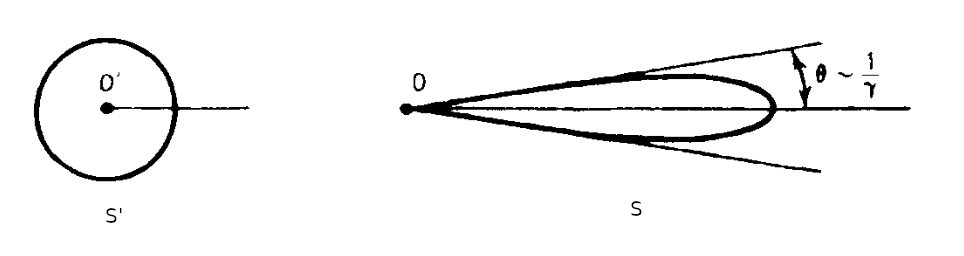
\includegraphics[width=\textwidth]{img/Beaming}
\caption{Schema dell'effetto di beaming relativistico.} \label{fig:Beaming}
\end{figure}

Studiamo ora il caso di una particella a riposo nel sistema $S'$ che emette fronte e retro. L'impulso medio della radiazione è perciò nullo, $\dd \V{p}'=0$. Pertanto la trasformazione del quadrivettore energia momento è semplicemnte $\dd W = \gamma \dd W'$. Inoltre vale $\dd t = \gamma \dd t'$, perciò la potenza è la stessa in entrambi i sistemi
\begin{equation}
\der{W}{t} = \der{W'}{t'} \label{eq:PotenzaInvariante}
\end{equation}
risultato valido solo nell'ipotesi di emissione fronte-retro. Questo risultato consente di usare la formula di Larmor nel sistema di riferimento $S'$, ottenendo
\begin{equation}
\der{W}{t} = \der{W'}{t'} = \dfrac{2}{3}\, \dfrac{q^2\, |\dot{v}'|^2}{c^3}
\end{equation}
Se $v'=0$, si può dimostrare che la trasformazione dell'accelerazione è 
\begin{align}
&a'_\| = \gamma^3 a_\|
&a'_\bot=\gamma^2 a_\bot
\end{align}
da cui si trova 
\begin{equation}
\der{W}{t} = \dfrac{2}{3} \dfrac{q^2}{c^3} \gamma^4 (a^2_\bot + \gamma^2 a^2_\|) \label{eq:Relatività2}
\end{equation}
che mostra che la potenza viene aumentata di un fattore $\gamma^4$ o $\gamma^6$ a seconda dell'accelerazione dominante.

Concludiamo questa sezione ricordando che la trasformazione di una quantità tensoriale è 
\begin{equation}
F'^{\mu\nu}= \Lambda_\sigma^\mu \Lambda_\tau^\nu F^{\sigma\tau}
\end{equation}

\subsection{Radiazione di sincrotrone}\label{subsec:Sincrotrone}
Il sincrotrone è la generalizzazione relativistica del ciclotrone, studiato nella sezione
\ref{subsec:Ciclotrone}. Avevamo ottenuto 
\begin{align}
&\der{W}{t} = 2\sigma_\mathrm{T} \,\beta^2\, c\, U_B = \dfrac{2}{3} \,r_0^2\,\beta^2 \,c \,B^2
&\omega_\mathrm{c} = \dfrac{qB}{mc}
\end{align}
con $U_B=B^2/8\pi$ e $\sigma_\mathrm{T}$ sezione d'urto Thomson. Per generalizzare questo risultato al caso relativistico consideriamo il fatto che la forza di Lorentz che agisce sulla particella non compie lavoro, poichè data solo dal campo magnetico ($\scal{F}{v}=0$). Pertanto l'energia cinetica della particella si conserva, e quindi $|\V{v}|=cost$, che a sua volta implica che $\gamma$ è costante. Possiamo scrivere la legge del moto della particella come\footnote{Il primo termine non è altro che la derivata della quantità di moto relativistica.}
\begin{equation}
\der{}{t}(\gamma m \V{v}) = \V{F} \,\,\,\,\,\,\,\,\,\,\,\,\,\,\, \Longrightarrow \,\,\,\,\,\,\,\,\,\,\,\,\,\,\, \gamma\der{}{t}(m \V{v}) = \V{F}
\end{equation}
Vediamo quindi che l'equazione del moto è la stessa del ciclotrone a meno del fattore gamma. La frequenza sarà la stessa del ciclotrone con l'aggiunta del fattore $\gamma$, ovvero
\begin{EQ}
\begin{equation}
\omega_\mathrm{s} = \dfrac{\omega_\mathrm{c}}{\gamma} = \dfrac{qB}{\gamma mc}
\end{equation}
\end{EQ}
A differenza del ciclotrone in cui abbiamo semplificato il moto della particella, viconlandola al piano ortogonale al campo magnetico, consideriamo ora il caso più generale di una particella con velocità data da una componente ortogonale e una parallela al campo magnetico, che generano così un moto elicoidale attorno al $\V{B}$, come mostrato nella figura \ref{fig:Sincrotrone}. Se definiamo $\alpha$ l'angolo compreso tra $\V{v}$ e $\V{B}$ detto \textit{pitch angle}, abbiamo
\begin{align}
&\begin{cases}
v_\bot = v\sin\alpha \\
v_\|=v\cos\alpha
\end{cases}
&\tan\alpha = \dfrac{v_\bot}{v_\|}
\end{align}
\begin{figure}
\begin{center}
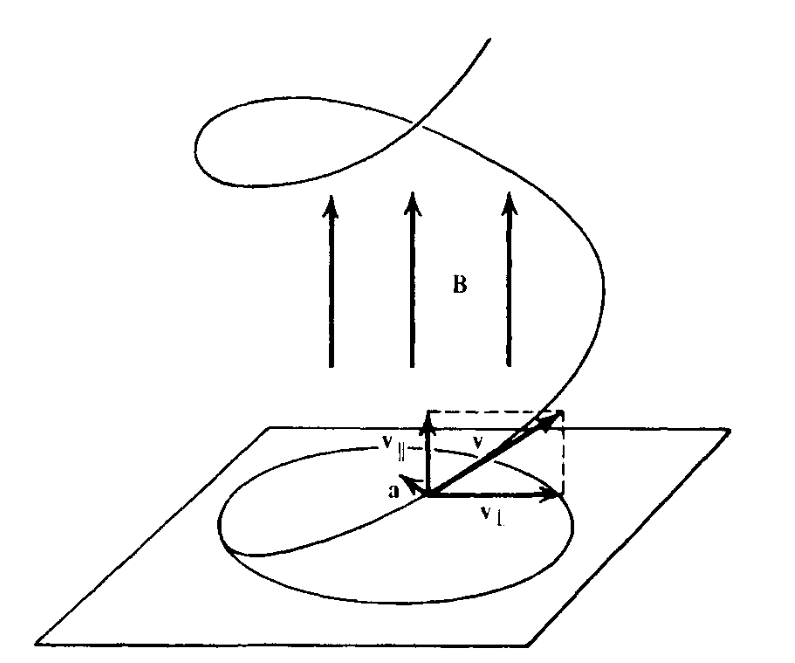
\includegraphics[width=0.8\textwidth]{img/Sincrotrone}
\caption{Moto elicoidale di una particella in un campo magnetico uniforme.} \label{fig:Sincrotrone}
\end{center}
\end{figure}
Per stimare la potenza emessa dalla radiazione di sincrotrone si procede analogamente a quanto fatto per il ciclottrone, solo che in questo caso la formula di Larmor iniziale è corretta per gli effetti relativistici, ed è data dalla \ref{eq:Relatività2}, in cui conta solo l'accelerazione ortogonale, quella parallela è nulla. Questo introduce inizialmente un fattore $\gamma^4$, mentre la frequenza di sincrotrone introduce un fattore $\gamma^{-2}$. Il risultato è quindi\footnote{Notiamo che nel regime non relativistico $\gamma\to 1$, mentre nel regime relativistico $\beta\to 1$. Perciò il prodotto $\gamma^2\beta^2$ si riduce a $\gamma^2$ nel regime relativistico, e a $\beta^2$ nel regime non relativistico, riducendosi al caso del ciclotrone.}
\begin{equation}
\der{W}{t} = 2\sigma_\mathrm{T} \, \gamma^2 \, \beta_\bot^2 \, c \, U_\mathrm{B} = \dfrac{2}{3} \,r_0^2\,\gamma^2\,\beta_\bot^2 \,c \,B^2 \label{eq:Sincrotrone1}
\end{equation}
con $\beta_\bot $ è il parametro $\beta$ riferito alla velocità ortogonale al campo magnetico. Lo possiamo quindi scrivere come $\beta_\bot = \beta \sin\alpha$. La popolazione degli elettroni avrà velocità orientate casualmente rispetto al campo magnetico, ciascuna delle quali sarà associata a un diverso fattore $\sin\alpha$. Pertanto è conveniente dare una stima della potenza totale come media su tutti i pitch angles della \ref{eq:Sincrotrone1}\footnote{Dobbiamo integrare il fattore $\sin^2\alpha$ su tutti gli angoli solidi e dividere per l'angolo solido totale \begin{align*}
<\sin^2\alpha> = \inv{4\pi}\int \sin^2\alpha\,\dd\Omega = \dfrac{2}{3}
\end{align*}}
ottenendo 
\begin{EQ}
\begin{equation}
<\der{W}{t}>_\mathrm{s} = \dfrac{4}{3}\,\sigma_\mathrm{T} \, \gamma^2 \, \beta^2 \, c \, U_B =  \dfrac{4}{9} \,r_0^2\,\gamma^2\,\beta^2 \,c \,B^2 \label{eq:Sincrotrone5}
\end{equation}
\end{EQ}
Resta ora da studiare lo spettro del sincrotrone. Iniziamo notando che quello di ciclotrone era molto semplice, una sola riga spettrale associata alla frequenza di ciclotrone. In questo caso si ha una complicazione dovuta al beaming relativistico; a causa di questo effetto l'elettrone emette essenzialmente lungo la tangente alla sua traiettoria, perciò vediamo la sua radiazione solo quando l'elettrone emette verso di noi. Quindi alla frequenza di sincrotrone $\omega_\mathrm{s}$ si aggiunge un'altra frequenza associata alla frequenza di visibilità della radiazione emessa. Discutiamo ora questo fenomeno in maniera più quantitativa.
\begin{figure}
\begin{center}
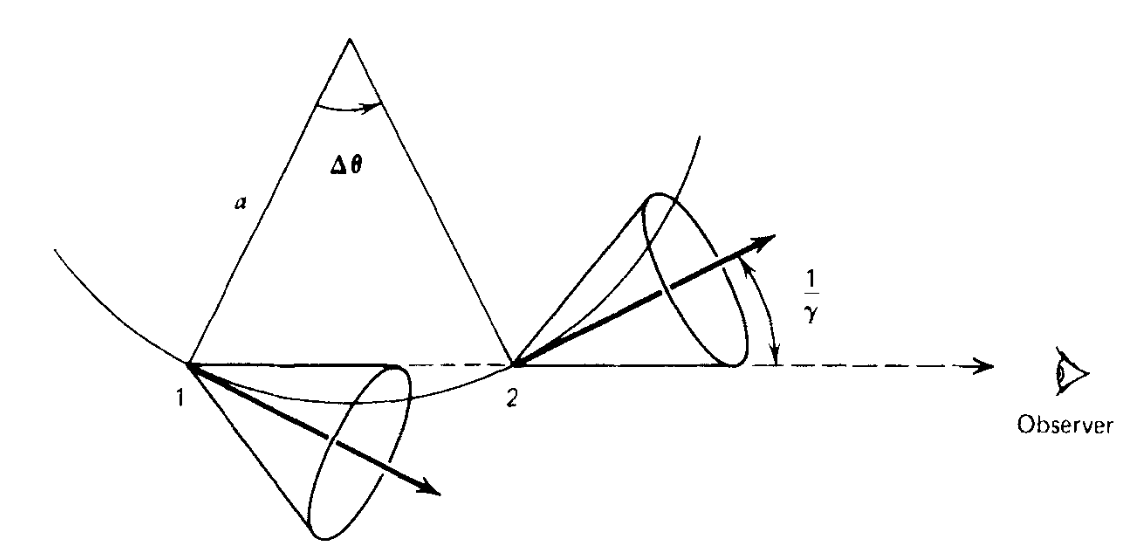
\includegraphics[width=0.8\textwidth]{img/Sincrotrone2}
\caption{Coni di emissione ai vari punti della traiettoria di una particella di sincrotrone.} \label{fig:Sincrotrone2}
\end{center}
\end{figure}
Facendo riferimento alla figura \ref{fig:Sincrotrone2} vediamo che quanto più è grande l'angolo di beaming tanto più e grande il tempo in cui è possibile osservare l'emissione dell'elettrone; la radiazione è infatti visibile quando il beam entra nella linea di vista fino a quando ne esce. Per evitare confusioni indichiamo con $r$ il raggio della traiettoria che in figura è indicato con $a$. Il tempo in cui la radiazione è visibile è
\begin{equation}
\Delta t_\mathrm{e} = \dfrac{r\Delta \theta}{v}
\end{equation}
Inoltre da semplici considerazioni geometriche risulta che\footnote{Il raggio di curvatura è dato da $r=\Delta s / \Delta\theta$ con $\Delta s$ pezzo di traiettoria tra i punti $1$ e $2$. L'equazione del moto 
\begin{align*}
\gamma m \dfrac{\Delta \V{v}}{\Delta t} = \dfrac{q}{c}\vett{v}{B}
\end{align*}
e il fatto che $|\V{v}| = v\Delta\theta$  e $\Delta s = v \Delta t $ permette di ottenere
\begin{align*}
\dfrac{\Delta \theta}{\Delta t} = \dfrac{qB\sin\alpha}{\gamma m c v}
\end{align*}
da cui segue l'espressione per $r$.}
\begin{align}
&r = \dfrac{v}{\omega_\mathrm{s} \sin\alpha}
&\Delta \theta = \dfrac{2}{\gamma}
\end{align}
e la differenza dei tempi di emissione si riduce a 
\begin{equation}
\Delta t_\mathrm{e} = \dfrac{2}{\gamma\omega_\mathrm{s}\sin\alpha}
\end{equation}
La differenza dei tempi di ricezione è data dalla differenza dei tempi di emissione meno il tempo che la radiazione impiega a percorrere il tragitto $\Delta s$, ovvero $r\Delta\theta /c$. Segue che la differenza dei tempi di ricezione, o detto in altri termini, la durata dell'impulso ricevuto è
\begin{equation}
\Delta t_\mathrm{r} = \dfrac{r\Delta\theta}{v}\left(1-\dfrac{v}{c}\right)
\end{equation}
Se $\gamma \gg 1$ allora possiamo approssimare\footnote{Si dimostra facilmente usando la relazione tra $\gamma$ e $\beta$.} $1-\beta \approx 1/2\gamma^2$, otteniamo
\begin{equation}
\Delta t_\mathrm{r} = \inv{\gamma^3 \omega_\mathrm{s} \sin\alpha} \equiv \inv{\omega_\mathrm{c}}
\end{equation}
Avremo quindi dgli impulsi di larghezza $1/\omega_\mathrm{c}$ che si ripetono dopo un tempo $1/\omega_\mathrm{s}$. Quindi passando al dominio delle frequenze avremo che la frequenza più piccola sarà $\omega_\mathrm{s}$, mentre quella più grande sarà $\omega_\mathrm{c}$ (dove $c$ sta per cono, non ciclotrone). 

Ottenere lo spettro è piuttosto complicato (non lo calcoleremo nel dettaglio), ma da un punto di vista qualitativo è più semplice. Se siamo in regime non relativistico abbiamo una singola frequenza, ovvero $\omega_\mathrm{s}$, e quindi lo spettro è una delta piccata su tale frequenza. Man mano che $v\to c$ compaiono anche le armoniche successive, a frequenze maggiori, fino a ottenere una foresta di frequenze che per $v\approx c$ diventa un inviluppo pressochè continuo, da $\omega_\mathrm{s}$ fino a $\omega_\mathrm{c}$. Notiamo che per come abbiamo definito $\omega_\mathrm{c}$ risulta che essendoci un fattore $\gamma^3$ di mezzo, $\omega_\mathrm{c}\gg\omega_\mathrm{s}$, e quindi le due frequenze differiscono tra loro anche per diversi ordini di grandezza (una velocità pari a $99\% c$ corrisponde a $\gamma=10$, e quindi ad una differenza tra le due frequenze di tre ordini di grandezza). 

Un modo relativamente semplice di vedere lo spettro è vederlo come la potenza emessa per unità di frequenza. Abbiamo calcolato la potenza emessa nella \ref{eq:Sincrotrone1} e possiamo usarla per stimare lo spettro: esso è dato da 
\begin{align*}
P(\omega) \equiv \der{P}{\omega}
\end{align*}
ma sappiamo che la scala naturale delle frequenze del problema è $\omega_\mathrm{c}$, quindi definendo una nuova variabile $x\equiv \omega/\omega_\mathrm{c}$, abbiamo che 
\begin{align*}
P(\omega) = \der{P}{x} \inv{\omega_\mathrm{c}}
\end{align*}
A questo punto esprimiamo la funzione $P(\omega)$ come un coeffieciente moltiplicato per una funzione di $x$
\begin{align*}
P(\omega) = P_0 f\left(\dfrac{\omega}{\omega_\mathrm{c}}\right)
\end{align*}
La funzione $f$ è adimensionale, mentre il coefficiente $P_0$ è una costante di proporzionalità tipica, che quindi stimiamo proprio come il rapporto tra la potenza totale e la frequenza $\omega_\mathrm{c}$. Si ottiene
\begin{equation}
P_0 \approx \dfrac{P}{\omega_\mathrm{c}} = \dfrac{2}{3} \, \dfrac{q^3\,B\,\sin\alpha}{m\, c^2}
\end{equation}
Il coefficiente $P_0$ descrive le scale tipiche dello spettro, il cui andamento esatto è descritto dalla funzione $f$, di cui non approfondiremo la forma (l'unica cosa che sappiamo è che quando il suo argomento supera il valore $1$ tende a zero rapidamente). Determinare la forma esatta di $f$ è in realtà superfluo, come mostreremo di seguito.

Finora abbiamo considerato un singolo elettrone e studiato il suo spettro. Se invece consideriamo più elettroni avremo una distribuzione di velocità degli elettroni, da cui dipende lo spettro totale molto più che dai singoli spettri degli elettroni. Infatti siccome lo spettro di singolo elettrone è funzione di $\omega_\mathrm{c}$ che a sua volta dipende fortemente dalla velocità, piccole differenze di velocità in una popolazione di elettroni fanno sì che si abbiano frequenze molto diverse tra loro nello spettro totale. In altre parole nella sovrapposizione dei singoli spettri conta molto di più la differenza tra le varie frequenze piuttosto che i profili $f$ dei singoli spettri. Vediamo questo concetto da un punto di vista quantitativo. Supponiamo che la popolazione degli elettroni segua una legge di potenza dell'energia $N(E)\,\dd E = C \, E^{-p} \, \dd E$\footnote{Se si ha una distribuzione di elettroni relativistici, tipicamente non si ha una popolazione termica, cioè la distribuzione delle velocità non è una Maxwelliana.}. Essendo l'energia dell'elettrone data da $E=\gamma m c^2$, la distribuzione delle velocità diventa
\begin{equation}
N(\gamma)\, \dd \gamma = C \gamma^{-p} \,\dd \gamma \label{eq:Sincrotrone2}
\end{equation}
ma è valida solo entro un certo troncamento, cioè per $\gamma_1 <\gamma < \gamma_2$ altrimenti se integriamo per ottenere il numero totale di particelle otteniamo un numero infinito. Calcoliamo ora lo spettro totale
\begin{equation}
P_\mathrm{tot} (\omega) = \int_{\gamma_1}^{\gamma_2} C \, P(\omega) \, \gamma^{-p} \, \dd\gamma \propto \int_{\gamma_1}^{\gamma_2} \, f\left(\dfrac{\omega}{\omega_\mathrm{c}}\right) \, \gamma^{-p} \, \dd\gamma
\end{equation}
Ricordando che $\omega_\mathrm{c} \propto 1/\gamma^3\omega_\mathrm{s} \propto \gamma^2$, cambiamo variabile in $x\equiv \omega/\omega_\mathrm{c}$ che implica $\dd\gamma \propto \omega^{1/2} \, x^{-3/2} \, \dd x$. Sotituendo si ricava
\begin{equation}
P_\mathrm{tot} (\omega) = \omega^{\frac{1-p}{2}} \int_{x_1}^{x_2} f(x) \, x^{\frac{p-3}{2}} \, \dd x
\end{equation}
con\footnote{A denominatore dovrebbe comparire $\sin\alpha$; di fattto non si ha un'uguaglianza ma una proporzionalità.}
\begin{align}
&x_1 = \dfrac{\omega}{\omega_\mathrm{ciclo}\gamma_2^2}
&x_2 = \dfrac{\omega}{\omega_\mathrm{ciclo}\gamma_1^2}
\end{align}
Se imponiamo che $x_1\ll 1$ e $x_2\gg 1$, ovvero 
\begin{equation}
\gamma_1^2 \omega_\mathrm{ciclo} \ll \omega \ll \gamma_2^2 \omega_\mathrm{ciclo}
\end{equation}
si ha che possiamo estendere gli estremi di integrazione a $0$ e $+\infty$; quindi dato che gli estremi di integrazione non dipendono più da $\omega$, l'integrale è anch'esso una costante, e quindi abbiamo trovato che la dipendenza dello spettro totale dalla frequenza è 
\begin{equation}
P_\mathrm{tot}(\omega) \propto \omega^\frac{1-p}{2} \label{eq:Sincrotrone4}
\end{equation}
Ecco perchè non è molto importante la forma dello spettro di singolo elettrone, ma lo è la distribuzione delle velocità.

Definiamo una quantità utile sperimentalmente, nota come \textit{indice spettrale} $s$
\begin{EQ}
\begin{equation}
s \approx -\der{(\ln P)}{(\ln\omega)}
\end{equation}
\end{EQ}
Viene così definito perchè solitamente in astronomia si riportano le misure di potenza in funzione della frequenza di osservazione, su grafici logaritmici. Se quindi abbiamo due misure, associate a due diverse frequenze, e vogliamo ottenere il coefficiente della retta che li congiunge, calcoliamo l'indice spettrale che appunto, per definizione, è l'inclinazione della retta che usnisce le due misure riportate nel suddetto grafico logaritmico. Nel caso del sincrotrone si ha
\begin{equation}
s=\dfrac{p-1}{2}
\end{equation}
ed è possibile misurare $p$ a partitre dall'indice spettrale\footnote{Questo è quello che si fa con le misure astronomiche in banda X. Tipicamente si hanno due bande, una \textit{hard} e una \textit{soft} in cui si contano i fotoni con dei rivelatori. Ciò consente di misurare la potenza in funzione della frequenza della banda. Dopodichè si ricava l'indice spettrale dalla retta che unisce i valori misurati nel grafico logaritmico che relaziona potenza e frequenza.}.
Così come abbiamo fatto per la bremsstrahlung dobbiamo considerare gli effetti dell'assorbimento a basse frequenze: la prima cosa da fare è ottenere il coefficiente di assorbimento. Per farlo usaimo la \textit{legge di Kirchhoff generalizzata}
\begin{EQ}
\begin{equation}
S_\nu = \dfrac{j_\nu}{\alpha_\nu} = \dfrac{2h\nu^3}{c^2}\left[ \dfrac{g_2\,n1}{g_1\,n_2} -1 \right]^{-1} \label{eq:Sincrotrone3}
\end{equation}
\end{EQ}
Il calcolo completo è piuttosto complicato; la legge di Kirchhoff generalizzata che abbiamo scritto è per il caso in cui si hanno due livelli energetici dell'elettrone, ma nel nostro caso ce ne sono molti più di due disponibili. Dovremmo considerare tutte le coppie di stati che hanno la stessa differenza di energia, e poi integrare su tutte le energie possibili. È evdente che determinare tutti questi stati e calcolarne la densità nello spazio delle fasi per poi integrare su tutto lo spazio delle fasi è un'operazione complessa, pertanto risolveremo il problema riducendoci ad un caso semplificato. 

Cambiamo il formalismo e consideriamo $\nu$, anzichè $\omega$ (il che è del tutto equivaleente, a meno di un fattore $2\pi$). Consideriamo due stati la cui differenza di energia è $\Delta E = h \nu$. Gli elettroni che emetterano a questa frequenza sono quelli che hanno $\nu_\mathrm{c}$ dell'ordine della frequenza del fotone emesso $\nu$. Ricordiamo che $\nu_\mathrm{c}\propto \gamma^2 \propto E^2$. Pertanto $E\propto\nu^{1/2}$. Poichè stiamo considerando assorbimento avremo $E_1=E$, mentre $E_2=E+h\nu$. Supponiamo ora che $g_2 = g_1$ cioè che i pesi statistici dei diversi livelli siano gli stessi. Ricordando la distribuzione che abbiamo assunto per gli elettroni (ovvero la \ref{eq:Sincrotrone2}) si ha che $n_1\propto E^{-p}$ mentre $n_2\propto (E+h\nu)^{-p}$. Poichè stiamo ipotizzando che il fotone considerato sia a basse frequenze (basse rispetto all'energia dell'elettrone che lo riassorbe) $h\nu \ll E$, quindi 
\begin{equation}
\dfrac{n_1}{n_2} \approx 1+ p\dfrac{h\nu}{E}
\end{equation}
Sostituendo nella \ref{eq:Sincrotrone3} si ottiene
\begin{equation}
S_\nu = \dfrac{2}{pc^2}\, \nu^2 \, E \propto \nu^{5/2}
\end{equation}
Per quanto visto nella \ref{eq:Sincrotrone4} risulta che 
\begin{equation}
j_\nu \propto \nu^\frac{1-p}{2}
\end{equation}
e che quindi 
\begin{equation}
\alpha_\nu \propto \nu^{-\frac{p+4}{2}}
\end{equation}
Tipicamente $p$ è sempre positivo, quindi per basse frequenze il coefficiente di assorbimento tende all'infinito; questo significa che esisterà sempre una frequenza critica al di sotto della quale il mezzo diventa otticamente spesso. In questo caso lo spettro tende alla funzione sorgente del mezzo, pertanto a basse frequenze lo spettro va come $\nu^{5/2}$, come si può vedere dalla figura \ref{fig:Sincrotrone3}. Se l'emissione fosse stata termica avremmo avuto una proporzionalità a $\nu^2$.
\begin{figure}
\begin{center}
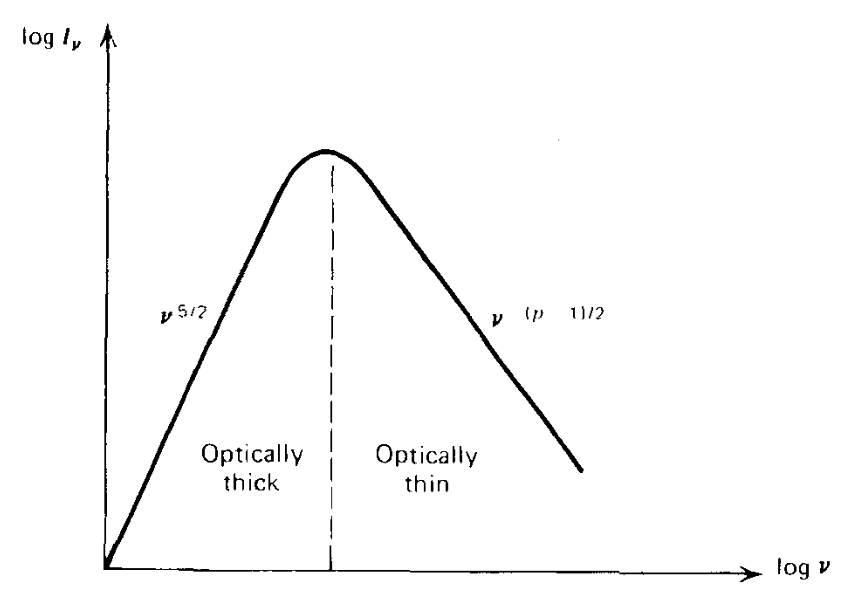
\includegraphics[width=0.8\textwidth]{img/Sincrotrone3}
\caption{Spettro di sincrotrone associato a una distribuzione a legge di potenza delle velocità degli elettroni.} \label{fig:Sincrotrone3}
\end{center}
\end{figure}

\subsection{Scattering Compton}
Lo scttering Compton è la versione relativistica dello scattering Thomson, studiato nella sezione \ref{subsec:Thomson} in cui avevamo ottenuto i seguenti risultati: lo scattering non dipende dalla frequenza (tutte le frequenze vengono scatterate nello stesso modo), la frequenza prima ($\nu$) e dopo ($\nu_1$) lo scattering è la stessa. Inoltre la sezione d'urto differenziale trovata era
\begin{equation}
\der{\sigma_\mathrm{T}}{\Omega}=\dfrac{r_0^2}{2}(1+cos^2\theta)
\end{equation}
con $\theta$ angolo di scattering e $r_0$ raggio classico dell'elettrone, mentre la sezione d'urto totale era
\begin{equation}
\sigma_\mathrm{T} = \dfrac{8\pi}{3}r_0^2
\end{equation}
Questi risultati sono validi nel regime non relativistico, per il quale vale $h\nu \ll \mel c^2$. Non affronteremo il calcolo della sezione d'urto nel caso relativistico poichè è piuttosto complicato e laborioso; ci limiteremo a ricavare la relazione tra la radiazione incidente e quella uscente. 

Nello scattering Compton si ha un fotone incidente su un elettrone libero e inizialmente fermo; a differenza dello scattering Thomson, l'energia del fotone è confrontabile con l'energia a riposo dell'elettrone, pertanto non si avrà più la conservazione dell'energia del fotone, bensì una conservazione del quadrivettore energia impulso del sistema. 
\begin{figure}
\begin{center}
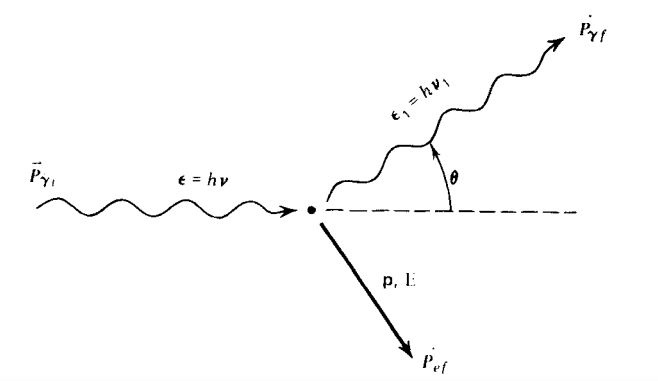
\includegraphics[width=0.8\textwidth]{img/Compton}
\caption{Schema dello scattering Compton.}
\end{center}
\end{figure}
Il fotone ha direzione iniziale $\vers{n}$ e direzione finale $\vers{n}_1$, direzioni che formano un angolo di scattering $\theta$. I quadrimomenti iniziali e finali dell'elettrone e del fotone sono
\begin{align}
&\V{p}_{\gamma_i} = \dfrac{h\nu}{c}(1,\,\vers{n})
&\V{p}_{\gamma_f} = \dfrac{h\nu_1}{c}(1,\,\vers{n}_1)
\end{align}
\begin{align}
&\V{p}_{e_i} = (\mel c, \, 0)
&\V{p}_{e_f} = (E/c,\,\V{p})
\end{align}
dove i pedici $\gamma$, $e$, $i$, $f$ indicano rispettivamente fotone, elettrone, iniziale, finale. La conservazione del quadrimomento implica che 
\begin{equation}
\V{p}_{e_f} = \V{p}_{\gamma_i} + \V{p}_{e_i} - \V{p}_{\gamma_f}
\end{equation}
Calcoliamo il modulo di questo quadrivettore\footnote{Il modulo quadro è dato dalla somma dei quadrati delle componenti spaziali, meno il quadrato della componente temporale (la prima componente)}, ottenendo
\begin{equation}
-\mel^2 c^2 = -\mel^2 c^2 + 2\quadre{-\mel h \nu + \mel h \nu_1 + \dfrac{h\nu_1 h \nu}{c^2} - \dfrac{h\nu_1 h \nu}{c^2} \cos\theta}
\end{equation}
che permette di ottenere
\begin{equation}
\nu_1 = \nu \quadre{1+\dfrac{h\nu}{\mel c^2}(1-\cos\theta)}^{-1} \label{eq:Compton1}
\end{equation}
Notiamo che $\nu_1<\nu$, cioè il fotone uscente ha energia minore di quello entrante, e che se $h\nu \ll \mel c^2$ ci si riduce al caso di scattering Thomson in cui la frequenza del fotone non cambia. Sfruttando questa relazione possiamo calcolare quant'è la variazione della lunghezza d'onda del fotone, ottenendo 
\begin{EQ}
\begin{equation}
\lambda_1 - \lambda = \lambda_\mathrm{C}(1-\cos\theta)
\end{equation}
\end{EQ}
con $\lambda_\mathrm{C}\equiv h/\mel c$ nota come \textit{lunghezza d'onda di Compton}. 

La sezione d'urto per lo scattering Compton è nota come \textit{sezione d'urto di Klein-Nishina}
\begin{EQ}
\begin{equation}
\der{\sigma}{\Omega}= \dfrac{r_0^2}{2}\tonde{\dfrac{\nu_1}{\nu}}^2 \quadre{\dfrac{\nu}{\nu_1}+\dfrac{\nu_1}{\nu}-\sin^2\theta} \label{eq:Compton2}
\end{equation}
\end{EQ}
Veidamo che nel regime non relativistico $h\nu\ll\mel c^2$ la \ref{eq:Compton1} implica che $\nu_1 \to \nu$, e quindila sezione d'urto di Klein-Nishina si riduce alla sezione d'urto differenziale di Thomson \ref{eq:Thomson4}\footnote{In questo paragrafo indichiamo l'angolo di scattering con $\theta$, mentre nella \ref{eq:Thomson4} è indicato con $\phi$.}. Definiamo il parametro
\begin{equation}
x \equiv \dfrac{h\nu}{\mel c}
\end{equation}
Le relazioni\ref{eq:Compton1} e \ref{eq:Compton2} permettono di descrivere lo scattering Compton. Vediamo che la sezione d'urto dipende dall'angolo di scattering $\theta$ e dalla frequenza del fotone incidente mediante il parametro $x$. Tale dipendenza implica che all'aumentare di $x$ cioè all'aumentare dell'energia del fotone icidente, la sezione d'urto si riduce sempre più rispetto al suo valore nel caso non relativistico. Inoltre nel regime Compton lo scattering retroverso, cioè associato a $\pi<\theta<\pi/2$, diventa sempre più trascurabile all'aumentare di $x$. L'andamento in funzione dell'angolo di scattering è riportato nella figura \ref{fig:Compton2}.
\begin{figure}[t!]
\begin{center}
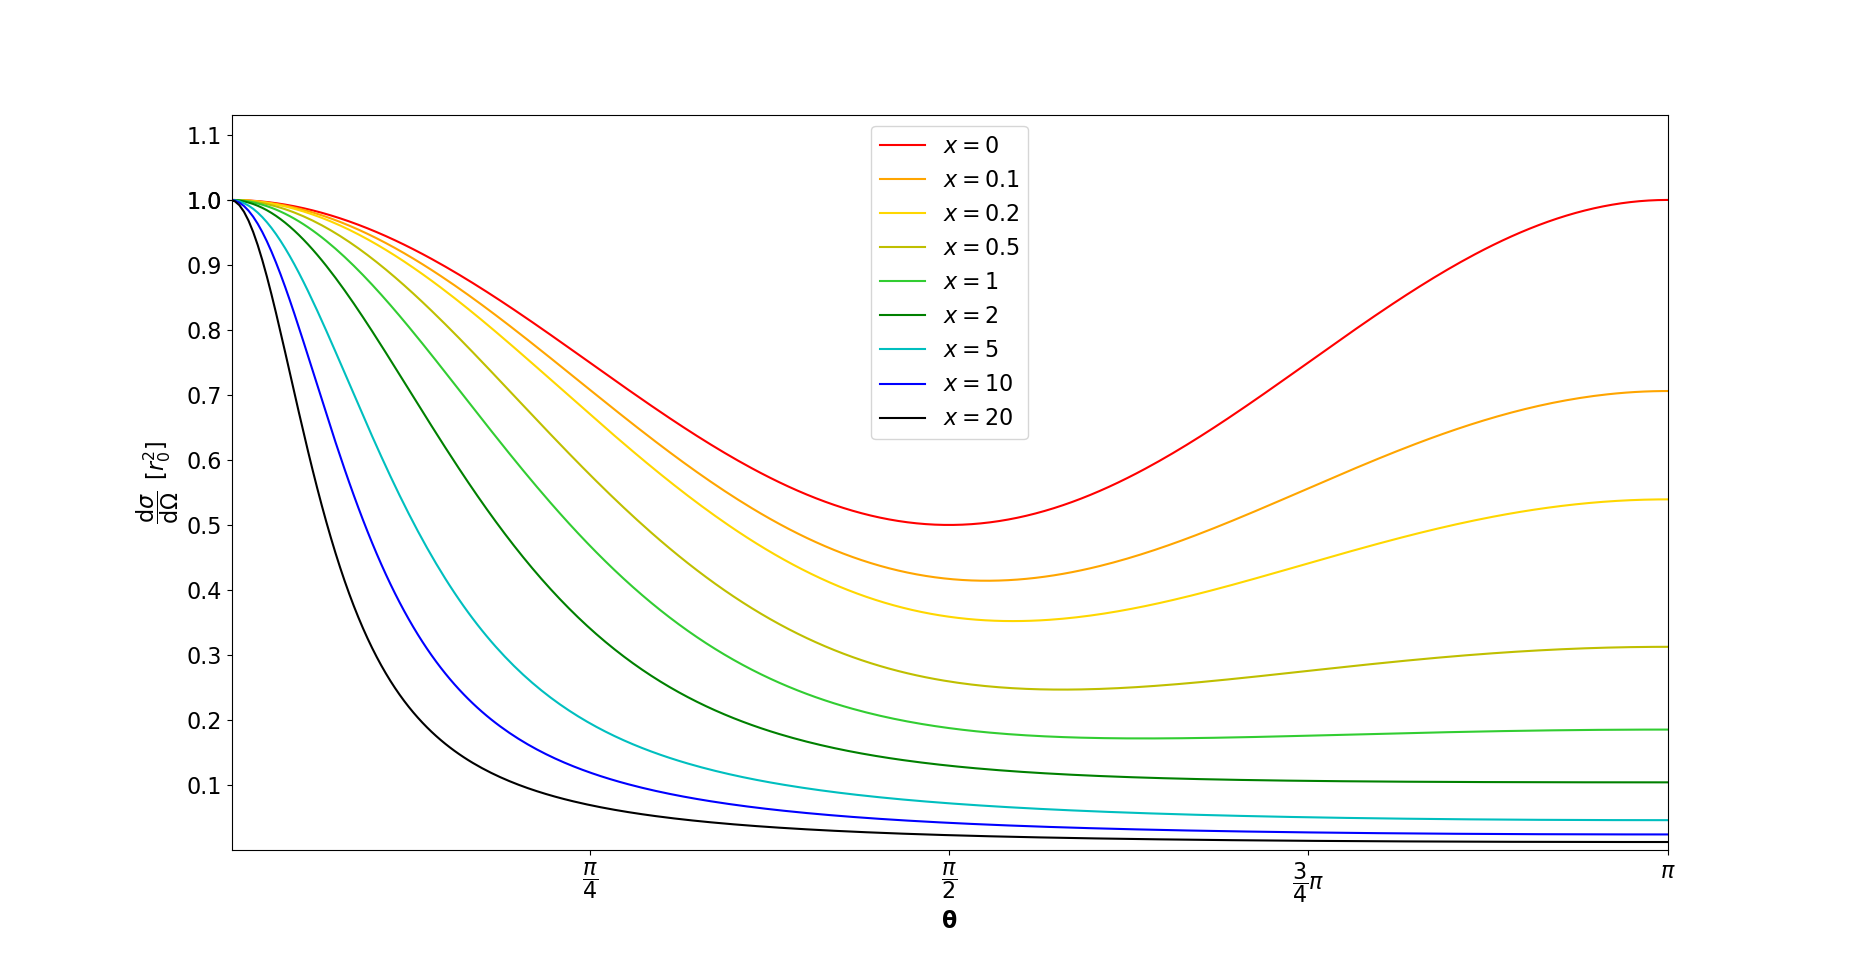
\includegraphics[width=\textwidth]{img/Compton2}
\caption{Andamento della sezione d'urto differenziale in funzione dell'angolo di scattering al variare del parametro $x$. Il caso $x=0$ è lo scattering Thomson.} \label{fig:Compton2}
\end{center}
\end{figure}

\subsection{Scattering Compton inverso}
Finora abbiamo considerato il caso di elettroni a riposo e fotoni energetici, ma tipicamente in astrofisica si hanno elettroni relativistici molto energetici che interagiscono con fotoni di bassa energia. In queste condizioni si ha \textit{scattering compton inverso} in quanto non è il fotone a trasferire energia all'elettrone, bensì il contrario. Questo processo va quindi ad aumentare l'energia del campo di radiazione, ed è perciò un processo di emissione. Mentre nello scattering Compton viene ridotta l'energia e quindi la frequenza del fotone, in questo caso il fotone aumenta la sua frequenza.

Per studiare questo problema distinguiamo i sistemi di riferimento $S$ in cui osserviamo l'elettrone relativistico che produce scattering Compton inverso, e il sistema $S'$ solidale con l'elettrone. Supponiamo che nel sistema $S$ il campo di radiazione sia isotropo, e quindi l'angolo di incidenza del fotone è un generico angolo $\theta$\footnote{Gli angoli sono definiti come compresi tra la direzione $\vers{x}$ del moto dell'elettrone, e la direzione di provenienza (o di uscita) del fotone.}. Nel sistema $S'$, a causa dell'effetto di beaming relativistico, l'angolo $\theta$ si trasforma nell'angolo $\theta'\approx\pi$. Nel sistema dell'elettrone si ha quindi un semplice scattering Compton/Thomson: ipotizziamo che lo scattering sia Thomson, potendo quindi assumere che l'angolo di emissione del fotone in questo sistema sia un generico $\theta'_1$\footnote{Ricordiamo che nella notazione usata il $'$ indica le grandezze misurate nel sistema solidale con l'elettrone, mentre il pedice $1$ indica le quantità dopo l'interazione fotone-elettrone.}. Se fosse scattering Compton avremmo una dipendenza dell'angolo di scattering dalla frequenza del fotone incidente, che complica la trattazione. Indichiamo con $\ecor$ l'energia del fotone nel sistema $S$; l'ipotesi di scattering Thomson in $S'$ implica che $\ecor' = \ecor'_1$. La trasformazione dell'energia dal sistema $S$ al sistema $S'$ è $\ecor' = \ecor\gamma(1-\beta\cos\theta)$, dove i parametri $\beta$ e $\gamma$ sono riferiti alla velocità dell'elettrone, poichè il sistema $S'$ è solidale all'elettrone. Infine si ha un effetto Doppler anche per l'energia del fotone uscente $\ecor_1 = \ecor'_1\gamma(1+\beta\cos\theta'_1)$. Unendo queste tre relazioni si ottiene
\begin{equation}
\ecor_1 = \ecor\gamma^2(1-\beta\cos\theta)(1+\beta\cos\theta'_1)
\end{equation}
Questa relazione può essere semplificata: sia $\theta$ che $\theta'_1$ non sono angoli estremi, sono due angoli generici. Pertanto (non è chiaro questo passaggio) i loro coseni assumeranno valori tipici dell'ordine dell'unità e quindi il prodotto delle due parentesi è anch'esso dell'ordine dell'unità. Quindi l'equazione si semplifica in $\ecor_1\approx\ecor\gamma^2$; l'effetto principale dello scattering Compton inverso è quindi un aumento dell'energia del fotone di un fattore $\gamma^2$.

Resta ora da determinare la potenza emessa per scattering Compton inverso. Per farlo iniziamo col fornire alcuni importanti risultati che non dimostreremo. Indichiamo con $n(p)$ la densità di fotoni nello spazio delle fasi ($p$ indica il modulo della quantità di moto dei fotoni) e con $f(\ecor)$ la densità dei fotoni nello spazio delle energie. Energia e quantità di moto del fotone sono legate, pertanto deve valere 
\begin{equation}
f(\ecor) \,\dd \ecor = n(p)\,\dd^3 p
\end{equation}
Si può dimostrare che da questa relazione e dal fatto che si può dimostrare che $n(p)$ è un'invariante di Lorentz, segue che 
\begin{equation}
\dfrac{f(\ecor) \,\dd \ecor }{\ecor} = \dfrac{f(\ecor') \,\dd \ecor' }{\ecor'}
\end{equation}
ovvero che la quantità riportata nell'equazione è un'invariante di Lorentz. Ricordiamo inoltre il risultato ottenuto nella \ref{eq:PotenzaInvariante}, ovvero che nel caso in cui nel sistema solidale con l'emettitore l'emissione ha simmetria fronte-retro, allora la potenza è un'invariante di Lorentz. Quest'ipotesi è soddisfatta poichè abbiamo assunto che nel sistema $S'$ solidale con l'elettrone si ha scattering Thomson, in quale è un processo che soddisfa questa simmetria.
Nel sistema di riferimento $S'$ si avrà che dopo l'interazione la potenza emessa è pari al flusso di energia dei fotoni incidenti sull'elettrone moltiplicato per la sezione d'urto Thomson. Da queste considerazioni si ha
\begin{align*}
\der{E_1}{t} &= \der{E'_1}{t'} = c\,\sigma_\mathrm{T}\int\ecor' f(\ecor')\,\dd\ecor' = 
c\,\sigma_\mathrm{T}\int \dfrac{\ecor'^2 f(\ecor')}{\ecor'}\,\dd\ecor' = \\
&= c\,\sigma_\mathrm{T}\int \gamma^2(1-\beta\cos\theta)^2 \dfrac{\ecor^2 f(\ecor')}{\ecor'}\,\dd\ecor' = \\
&= c\,\sigma_\mathrm{T}\int \gamma^2(1-\beta\cos\theta)^2 \dfrac{\ecor^2 f(\ecor)}{\ecor}\,\dd\ecor =\footnotemark \\
&=c \,\sigma_\mathrm{T}\gamma^2 <(1-\beta\cos\theta)^2> \, U_\mathrm{ph} = \\
&= c \sigma_\mathrm{T}\gamma^2\tonde{1+\dfrac{\beta^2}{3}} U_\mathrm{ph}
\end{align*}
\footnotetext{La variabile $\theta$ dipende dall'energia e quindi va tenuta dentro all'integrale, che se non fosse per il fattore tra parentesi coincide con la densità di energia dei fotoni. Si può aggirare questo problema sostituendo il termine in $\theta$ con il suo valor medio su tutto l'angolo solido. L'angolo è infatti generico, quindi possiamo fare l'apporssimazione di sostituirlo con il suo valor medio, di modo da semplificare il calcolo.}
Abbiamo così ottenuto una stima per la potenza del campo di radiazione dopo lo scattering Compton inverso
\begin{equation}
\der{E_1}{t}  =c \sigma_\mathrm{T}\gamma^2\tonde{1+\dfrac{\beta^2}{3}} U_\mathrm{ph}
\end{equation}
Per trovare la potenza fornita ai fotoni per effetto Compton inverso basta sottrarre a questa quantità, la potenza che i fotoni avevano inizialmente prima di interagire con l'elettrone. Si ottiene facilmente\footnote{
\begin{align*}
P_\mathrm{IC} = \der{E_1}{t} - \der{E}{t}  = c\,\sigma_\mathrm{T} \, U_\mathrm{ph} \tonde{\gamma^2-1+\dfrac{\beta^2\gamma^2}{3}} = c\,\sigma_\mathrm{T} \, U_\mathrm{ph} \tonde{\beta^2\gamma^2+\dfrac{\beta^2\gamma^2}{3}} = \dfrac{4}{3} \, c\,\sigma_\mathrm{T}\,\gamma^2\,\beta^2\,U_\mathrm{ph}
\end{align*}}
\begin{EQ}
\begin{equation}
P_\mathrm{IC} = \dfrac{4}{3} \, c\,\sigma_\mathrm{T}\,\gamma^2\,\beta^2\,U_\mathrm{ph}
\end{equation}
\end{EQ}
Notiamo che il risultato è del tutto simile a quello ottenuto per la radiazione di sincrotrone \ref{eq:Sincrotrone5}. I due processi sono infatti analoghi: nel Compton inverso si ha interazione di elettroni relativistici con un campo elettromagnetico (variabile nel tempo), mentre nel caso del sincrotrone si ha interazione di elettroni relativistici con un campo magnetico statico. In entrambi i casi si hanno elettroni relativistici che interagiscono con dei fotoni, solo che tali fotoni sono reali nel primo caso, e virtuali nel secondo. Se quindi si ha un sistema in cui sono presenti sia un campo di radiazione che un campo magnetico statico, si può calcolare il rapporto tra la potenza emessa dalla radiazione di sincrotrone e da quella di Compton inverso come il rapporto delle densità energetiche associate al campo magnetico e al campo di radiazione elettromagnetica
\begin{equation}
\dfrac{P_\mathrm{s}}{P_\mathrm{IC}} = \dfrac{U_\mathrm{B}}{P_\mathrm{ph}} 
\end{equation}
Per avere un'idea di quanto aumenta l'energia di un fotone per Compton inverso, consideriamo un fattore $\gamma=10^3$. In tal caso si ha
\begin{align*}
\mathrm{Radio}\,\,\nu\approx 10^{9} \uHz{} \,\,\,\,\,\,\,\,\,\,\,\,\,\,\,&\longrightarrow\,\,\,\,\,\,\,\,\,\,\,\,\,\,\, \mathrm{UV} \,\,\nu\approx 10^{15} \uHz{} \\
\mathrm{IR}\,\,\nu\approx 10^{12} \uHz{} \,\,\,\,\,\,\,\,\,\,\,\,\,\,\,&\longrightarrow\,\,\,\,\,\,\,\,\,\,\,\,\,\,\, \mathrm{X} \,\,\nu\approx 10^{18} \uHz{} \\
\mathrm{Ottico}\,\,\nu\approx 10^{14} \uHz{} \,\,\,\,\,\,\,\,\,\,\,\,\,\,\,&\longrightarrow\,\,\,\,\,\,\,\,\,\,\,\,\,\,\, \gamma \,\,\nu\approx 10^{20} \uHz{} 
\end{align*}
Il principale meccanismo di produzione di fotoni $\gamma$ in astrofisica è proprio tramite Compton inverso. un esempio sono i \textit{gamma ray burst}. 
Un esempio processo astrofisico tipico che sfrutta il Compton inverso è il \textit{self synchro-compton}. Il sistema è costituito da un sistema di elettroni relativistici in un campo magnetico, grazie al quale si genera radiazione di sincrotrone. I fotoni prodotti subiscono poi scattering Compton inverso dagli stessi elettroni relativistici che li hanno prodotto. Si ha così uno spettro di sincrotrone traslato a frequenze maggiori di un fattore $\gamma^2$. Sistemi del genere sono le \textit{Blazar} ovvero buchi neri da cui si genera un getto di elettroni relativistici, e i \textit{gamma ray burst}.
Un altro processo in cui interviene lo scattering Compton inverso, è l'\textit{effetto Sunyaev-Zeldovich}. Esso non è altro che scattering Compton inverso fatto da gas caldo sui fotoni del \textit{fondo cosmico a microonde}, noto come CMB. Il gas caldo che produce questo effetto si trova negli ammassi di galassie; questo gas oltre a produrre questo effetto, produce di per sè bremsstrahlung.

\begin{figure} 
\begin{center}
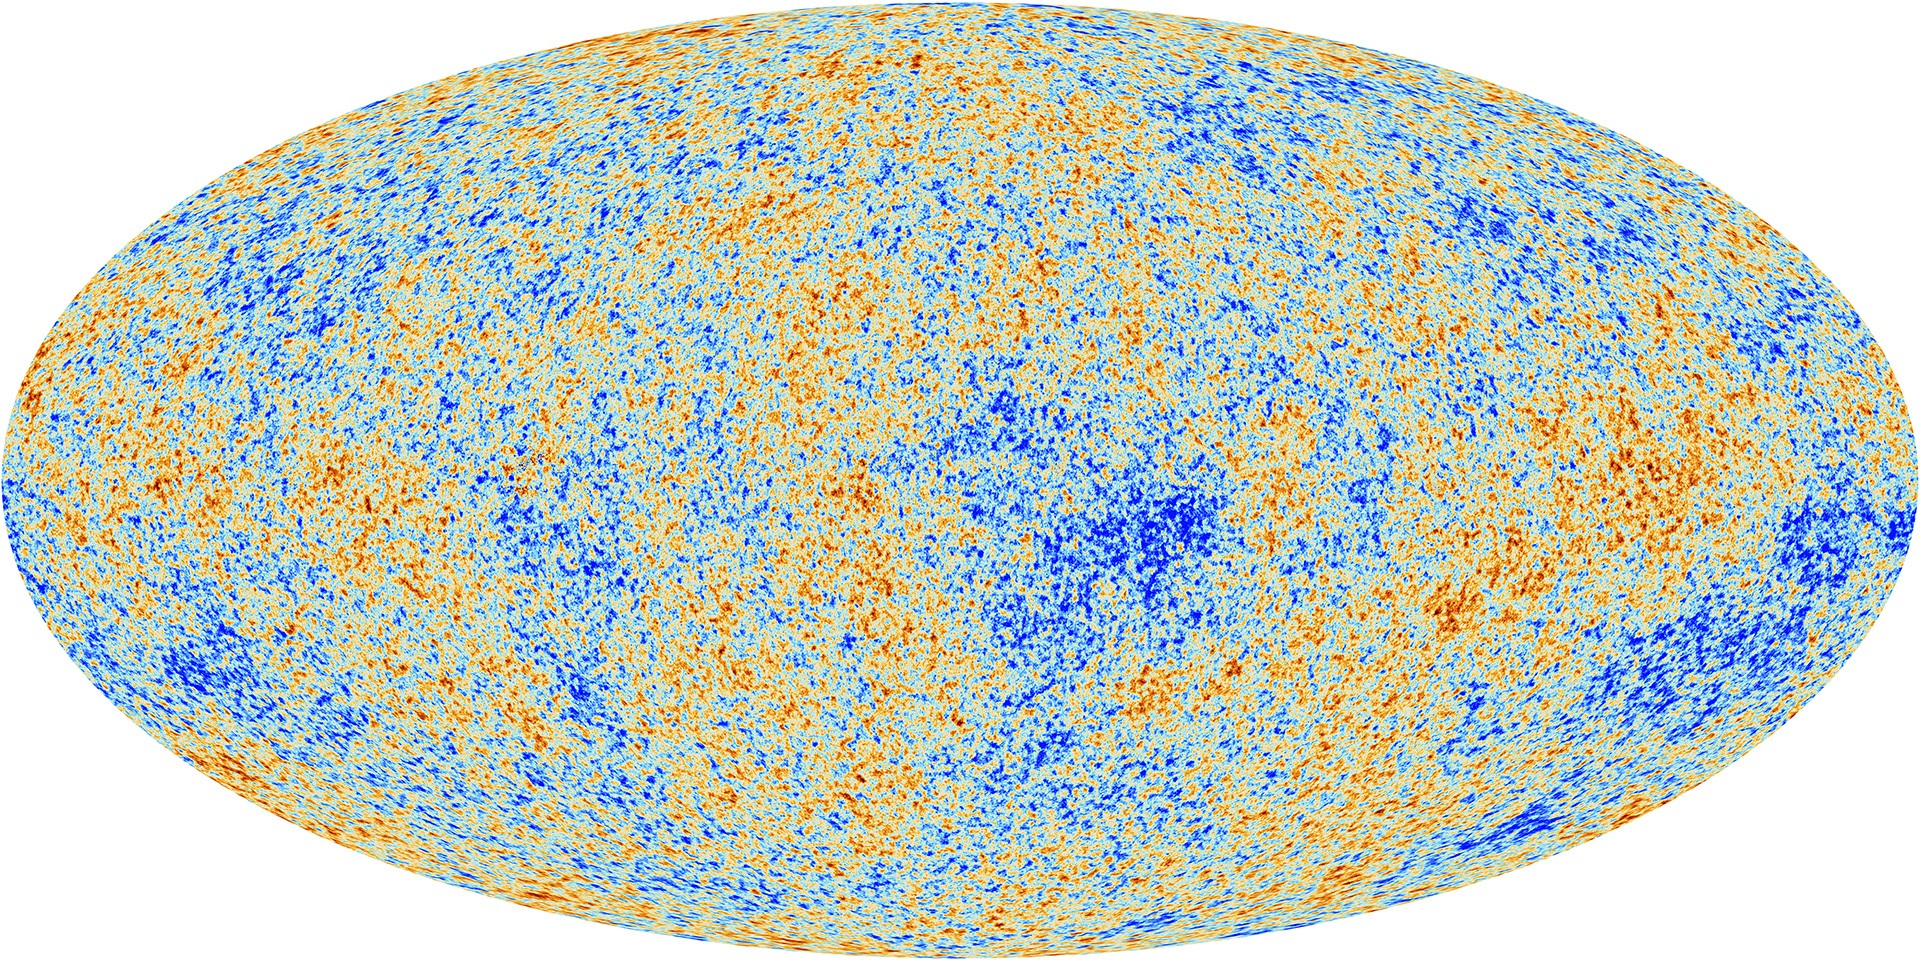
\includegraphics[width=0.8\textwidth]{img/CMB}
\caption{Radiazione di fondo cosmico a microonde.}
\end{center}
\end{figure}

Concludiamo questa sezione presentando un parametro che viene utilizzato per determinare se un sistema fa effetto Comton inverso o no. Come abbiamo visto, nel Compton inverso la variazione di frequenza dei fotoni è dell'ordine di $\gamma^2\beta^2$\footnote{Lo si può vedere dal fatto che $\nu_\mathrm{f}-\nu_\mathrm{i} \approx \gamma^2\nu_\mathrm{i}-\nu_\mathrm{i} = \gamma^2\beta^2\nu_\mathrm{i}$. Segue che $\Delta\nu/\nu \approx \gamma^2\beta^2$}. Per la precisione si ha
\begin{equation}
\dfrac{\Delta\nu}{\nu} = \dfrac{4}{3}\gamma^2\beta^2 \to 
\begin{cases}
\dfrac{4}{3}\beta^2 \,\,\,\,\,\,\,\,\,\,\,\,\,\,\,\,\,\,\,\,\beta\ll 1\\[10pt]
\dfrac{4}{3}\gamma^2 \,\,\,\,\,\,\,\,\,\,\,\,\,\,\,\,\,\,\,\,\beta\gg 1
\end{cases}
\end{equation}
Supponiamo di avere una popolazione termica di elettroni in equilibrio termico. Si ha che 
\begin{equation}
<\beta^2> = \dfrac{2}{2}<\dfrac{\mel v^2}{\mel c^2}> = \dfrac{3kT}{\mel c^2}
\end{equation}
per il caso non relativistico, mentre per il caso relativistico si ha
\begin{equation}
<\gamma^2 > = <\tonde{\dfrac{E}{\mel c^2}}^2> = 12 \tonde{\dfrac{kT}{\mel c^2}}^2
\end{equation}
Otteniamo quindi
\begin{equation}
<\dfrac{\Delta\nu}{\nu}> = 
\begin{cases}
\dfrac{4kT}{\mel c^2} \,\,\,\,\,\,\,\,\,\,\,\,\,\,\,\,\,\,\,\,\beta\ll 1\\[10pt]
\tonde{\dfrac{4kT}{\mel c^2}}^2 \,\,\,\,\,\,\,\,\,\,\,\,\,\,\,\,\,\,\,\,\beta\gg 1
\end{cases}\label{eq:ComptonInverso1}
\end{equation}
Vediamo quindi che per valutare l'importanza dell'effetto Compton, occorre misurare il parametro $\Delta\nu/\nu$, che dipende da $T$ nel caso non relativistico di scattering Thomson, e da $T^2$ nel caso relativistico di scattering Compton inverso. In realtà questo risultato è valido per un solo scattering. Nel caso generale si hanno scattering multipli e il sistema è quindi nel regime otticamente spesso. Questo ci fa intuire che l'importanza degli scattering multipl è legata al valore dello spessore ottico Thomson, ovvero $\tau_\mathrm{e}=n\sigma_\mathrm{T} R$ con $R$ dimensione tipica del mezzo. Il risultato \ref{eq:ComptonInverso1} va modificato, moltiplicandolo per $\mathrm{max}[\tau_\mathrm{e}, \,\tau_\mathrm{e}^2]$; infatti se si hanno pochi scattring l'energia (e quindi la frequenza) va pesata con la probabilità di fare uno scattering, ovvero $\tau_\mathrm{e}$. Se si hanno molti scattering si ha un processo non lineare, in cui conta il quadrato della densità dei bersagli, e quindi la probabilità di scattering sarà $\tau_\mathrm{e}^2$. Si definisce un parametro $y$ detto \textit{parametro di comptonizzazione}, che interpola i regimi relativistico e non relativistico
\begin{EQ}
\begin{equation}
y \equiv \dfrac{\Delta\nu}{\nu} =  \dfrac{4kT}{\mel^2}\tonde{1+\dfrac{4kT}{\mel^2}}\,\mathrm{max}[\tau_\mathrm{e}, \,\tau_\mathrm{e}^2]
\end{equation}
\end{EQ}